\documentclass[11pt,a4paper]{article}

% Required packages
\usepackage[utf8]{inputenc}
\usepackage[T1]{fontenc}
\usepackage{amsmath,amssymb,amsfonts}
\usepackage{graphicx}
\usepackage[margin=2.5cm]{geometry}
\usepackage{booktabs}
\usepackage{array}
\usepackage{multirow}
\usepackage{url}
\usepackage[hidelinks]{hyperref}
\usepackage[numbers]{natbib}
\usepackage{times}
\usepackage{lineno}
\usepackage{setspace}
\usepackage{fancyhdr}

% Fix header height
\setlength{\headheight}{14pt}

% Page setup
\pagestyle{fancy}
\fancyhf{}
\rhead{\thepage}
\lhead{Heat-Health Pathways in Johannesburg}

% Title and authors
\title{\textbf{Uncovering Heat-Health Pathways in Johannesburg: An Explainable Machine Learning Approach Using Harmonized Urban Cohort Data}}

\author{
Craig Parker$^{1,*,\dagger}$, Matthew Chersich$^{1,\dagger}$, Nicholas Brink$^{1}$, Ruvimbo Forget$^{1}$,\\
Kimberly McAlpine$^{1}$, Marié Landsberg$^{1}$, Christopher Jack$^{2}$,\\
Yao Etienne Kouakou$^{3,4}$, Brama Koné$^{3,4}$, Sibusisiwe Makhanya$^{5}$,\\
Etienne Vos$^{5}$, Stanley Luchters$^{6,7}$, Prestige Tatenda Makanga$^{6,8}$,\\
Guéladio Cissé$^{4}$\\[0.5cm]
\small
$^{1}$ Wits Planetary Health Research, Faculty of Health Sciences, University of the Witwatersrand,\\
\quad Johannesburg 2193, South Africa\\
$^{2}$ Climate System Analysis Group, University of Cape Town, Cape Town 7700, South Africa\\
$^{3}$ University Peleforo Gon Coulibaly, Korhogo BP 1328, Côte d'Ivoire\\
$^{4}$ Centre Suisse de Recherches Scientifiques, Abidjan 01 BP 1303, Côte d'Ivoire\\
$^{5}$ IBM Research—Africa, Johannesburg 2157, South Africa\\
$^{6}$ Centre for Sexual Health and HIV \& AIDS Research (CeSHHAR), Harare, Zimbabwe\\
$^{7}$ Liverpool School of Tropical Medicine, Liverpool L3 5QA, UK\\
$^{8}$ Surveying and Geomatics Department, Midlands State University, Gweru, Zimbabwe\\[0.3cm]
$^{*}$ Correspondence: craig.parker@wits.ac.za; Tel.: +27-11-717-2000\\
$^{\dagger}$ These authors contributed equally to this work.
}

\date{\today}

\begin{document}

\maketitle

\begin{abstract}
\textbf{Background:} Climate change disproportionately affects urban populations in sub-Saharan Africa, yet the complex pathways linking heat exposure, socioeconomic factors, and health outcomes remain poorly understood. Traditional epidemiological approaches cannot capture the multi-domain interactions necessary for developing targeted climate adaptation strategies.

\textbf{Methods:} We applied explainable machine learning to analyze heat-health relationships using harmonized data from 2,334 participants across multiple Johannesburg cohorts (2013--2021). Climate data (ERA5, WRF, MODIS, SAAQIS; 67 variables) and socioeconomic indicators (GCRO Quality of Life surveys; 73 variables) were temporally linked with seven standardized biomarkers. XGBoost, Random Forest, and Gradient Boosting models with SHAP analysis quantified feature importance and interaction effects across 1--90 day exposure windows.

\textbf{Results:} Glucose metabolism demonstrated exceptional climate predictability (R² = 0.611), with 21-day temperature exposure windows optimal for prediction. SHAP analysis revealed climate variables contributed 45\% of prediction importance, socioeconomic factors 32\%, with critical Age × Temperature interactions. A 1,300-fold heat vulnerability gradient was identified across the population, with housing quality contributing 42\% to vulnerability indices. Gender-specific responses showed females exhibiting 62\% greater glucose sensitivity to sustained heat exposure.

\textbf{Conclusions:} This study provides the first quantified heat-health-socioeconomic pathway analysis for African urban populations. The 21-day optimal exposure windows challenge existing early warning systems focused on acute heat events. The evidence-based vulnerability framework enables precision targeting of climate health interventions, with glucose monitoring emerging as a key indicator for heat-health surveillance systems.

\textbf{Keywords:} climate health; heat exposure; machine learning; SHAP analysis; urban health; socioeconomic vulnerability; glucose metabolism; African populations; explainable AI
\end{abstract}

\doublespacing
\linenumbers

\section{Introduction}

Climate change poses unprecedented health risks to urban populations in sub-Saharan Africa, where rapid urbanization intersects with increasing temperature extremes \cite{watts2021lancet,romanello2022lancet}. Continental-scale projections estimate that up to 2 billion urban Africans will be exposed to extreme heat events by 2100, with South African cities among the most vulnerable \cite{fotsonguemo2023projected}. Heat exposure affects human health through multiple physiological pathways, including cardiovascular stress, dehydration, and metabolic dysfunction, with impacts modified by individual vulnerability factors and environmental conditions \cite{hajek2022heat,li2022heat}. However, the complex interactions between climate exposure, socioeconomic circumstances, and health outcomes remain inadequately characterized, particularly in African urban contexts where traditional Western-derived risk models may not apply \cite{robinson2021african}.

The problem is multifaceted and deeply rooted in urban spatial legacies. African cities face a dual burden of infectious and non-communicable diseases, which may exacerbate heat vulnerability by compromising adaptive capacity \cite{khine2023implications,manyuchi2022extreme}. In South African contexts specifically, evidence demonstrates 1\% mortality increase per 1°C temperature rise in urban areas \cite{scovronick2018association,wichmann2017heat}, yet spatially explicit vulnerability mapping remains limited despite extreme socio-spatial inequality.

Johannesburg, South Africa's economic hub with over 5.9 million residents, exemplifies these challenges through its unique vulnerabilities. Its high altitude creates distinctive thermal dynamics that differ from coastal urban heat patterns \cite{naicker2017indoor}; its apartheid legacy has produced extreme spatial inequality in heat exposure and adaptive capacity, with informal settlements experiencing disproportionate heat impacts \cite{strauss2019historical,ansah2024climate}; and its rapidly changing urban form creates new thermal hot spots faster than understanding can keep pace \cite{simwanda2019spatial}. The city exhibits significant socioeconomic gradients, from affluent suburban areas to dense informal settlements, with temperature differentials of approximately 6°C between affluent neighbourhoods and informal settlements, and housing quality further exacerbating disparities with informal dwellings experiencing indoor temperatures up to 15°C higher than formal housing \cite{naicker2017indoor,souverijns2022urban}. Previous studies have documented temperature-health associations in South African populations \cite{wright2014human,wichmann2017heat}, but these have largely relied on ecological approaches that cannot capture individual-level mechanisms or identify optimal intervention targets.

Traditional epidemiological methods face several limitations when analyzing climate-health relationships, particularly what we term the "temperature fallacy"—the assumption that heat exposure alone determines vulnerability, failing to capture the social dimensions that determine who suffers during heat events. Standard regression approaches assume linear relationships and additive effects, failing to capture the non-linear interactions characteristic of climate-health pathways \cite{gasparrini2015mortality}. Time-series analyses typically examine short-term associations, missing the cumulative effects of sustained heat exposure that may be more relevant for physiological adaptation and health outcomes \cite{armstrong2014models}. Furthermore, socioeconomic modification of climate-health relationships is often treated as a confounder rather than an integral component of the causal pathway \cite{reid2009mapping}. Most applications have relied on global statistical methods that assume spatial stationarity—a problematic assumption for cities like Johannesburg with extreme socio-spatial inequality \cite{harris2011geographically}.

Machine learning approaches offer new opportunities to address these limitations. Tree-based ensemble methods can capture non-linear relationships and complex interactions without requiring a priori specification of functional forms \cite{chen2016xgboost,breiman2001random}. However, the "black box" nature of these algorithms has limited their application in health research, where mechanistic understanding is crucial for intervention development \cite{murdoch2019definitions}.

Recent advances in explainable artificial intelligence (XAI), particularly SHAP (SHapley Additive exPlanations) analysis, enable decomposition of model predictions into individual feature contributions while maintaining theoretical foundations in cooperative game theory \cite{lundberg2017unified}. This approach has shown promise in clinical applications \cite{chen2020machine} but has not been systematically applied to climate-health research, particularly in African contexts.

The present study addresses this gap by applying explainable machine learning to quantify heat-health-socioeconomic pathways using harmonized multi-cohort data from Johannesburg, informed by a novel 'spatial-temporal heat vulnerability' framework that advances environmental inequality scholarship by operationalising explicit connections between historical spatial development patterns and contemporary heat exposure. We hypothesized that: (1) machine learning models would reveal non-linear heat-health relationships not captured by traditional methods; (2) socioeconomic factors would modify these relationships through identifiable interaction patterns; (3) optimal exposure windows for health prediction would differ from those used in current early warning systems; and (4) SHAP analysis would identify actionable targets for climate health interventions. Our approach recognises that heat vulnerability is not simply about temperature—it is fundamentally about power, access, and historical patterns of urban development that continue to shape who lives and who dies during extreme heat events.

\section{Materials and Methods}

\subsection{Study Design and Setting}

This cross-sectional analysis utilized harmonized data from multiple cohorts in Johannesburg, South Africa (26.2041°S, 28.0473°E), collected between 2013 and 2021. Johannesburg is characterized by distinct urban heat island effects, with temperature variations of up to 5°C between urban core and periphery areas \cite{jury2021johannesburg}, and recent high-resolution analysis demonstrating that heat stress clusters in areas with high building density and low vegetation, often coinciding with lower socioeconomic areas \cite{souverijns2022urban}. The city exhibits extreme socioeconomic inequality, with Gini coefficients exceeding 0.75 in some areas \cite{gcro2016quality}. The spatial patterns of vulnerability are not random but reflect deliberate planning decisions made during the apartheid era that continue to influence contemporary heat exposure, with wealthy areas benefiting from mature tree canopies and thermally efficient building designs, while townships and informal settlements face intensified urban heat islands due to dense construction, heat-retaining materials, and limited cooling infrastructure \cite{knox2017postapartheid,chen2024inequality}.

Study protocols were approved by the University of the Witwatersrand Human Research Ethics Committee (HREC) under protocol M170837. All participants provided written informed consent in their preferred language (English, Zulu, Sotho, or Afrikaans).

\subsection{Study Population and Data Harmonization}

Data were integrated from eight cohort studies conducted by Wits Planetary Health Research and collaborating institutions: DPHRU-053 (Diabetes Prevention and Healthy Urban Living, n=456), VIDA-008 (Violence, Injury, Disability, and Ageing, n=312), JHB-EZIN-002 (Economic Zone Infrastructure and Health, n=189), JHB-IMPAACT-010 (International Maternal Pediatric Adolescent AIDS Clinical Trials, n=267), JHB-SCHARP-006 (Statistical Center for HIV/AIDS Research and Prevention, n=423), JHB-VIDA-007 (Violence and Injury Disability Assessment, n=298), JHB-WRHI-003 (Wits Reproductive Health and HIV Institute, n=234), and WRHI-001 (Wits Reproductive Health Institute Biomarker Study, n=155). Harmonization protocols standardized demographic variables, geographic coordinates, temporal linkage, and biomarker measurements across cohorts, enabling investigation of heat-health relationships across multiple physiological systems while maximising statistical power and demographic representation \cite{macleod2022cohort}. Participants with missing geographic coordinates, key demographic data, or biomarker values were excluded, resulting in a final analytic sample of 2,334 individuals.

\subsection{Health Outcome Measures}

Seven standardized biomarkers were selected based on evidence for heat sensitivity and clinical relevance: fasting glucose, glycated hemoglobin (HbA1c), systolic and diastolic blood pressure, serum potassium, blood urea nitrogen, and hemoglobin. All biomarkers were standardized using z-score transformation to enable cross-cohort comparison and model interpretation.

\subsection{Climate Data Integration}

Four complementary climate datasets provided comprehensive exposure characterization: ERA5 Reanalysis (hourly 2-meter air temperature, relative humidity, wind speed, and solar radiation at 0.25° resolution), Weather Research and Forecasting (WRF) Model (high-resolution 1 km temperature and humidity fields), MODIS Land Surface Temperature (8-day composite thermal infrared observations at 1 km resolution), and South African Air Quality Information System (SAAQIS) ground-based meteorological observations.

Climate variables were extracted for participant residential coordinates across temporal windows ranging from 1 to 90 days prior to biomarker collection, generating 67 unique exposure metrics per participant.

\subsection{Machine Learning Pipeline}

Three ensemble machine learning algorithms were implemented following established best practices for climate-health applications \cite{basu2018machine,hirano2021machine}: XGBoost (Extreme Gradient Boosting) for optimized gradient boosting with regularization techniques to prevent overfitting \cite{chen2016xgboost}, Random Forest (ensemble of decision trees with bootstrap aggregation and random feature selection) for robustness \cite{breiman2001random}, and Gradient Boosting (sequential ensemble method building models iteratively to correct predecessor errors) \cite{friedman2001greedy}. Model hyperparameters were optimized using 5-fold cross-validation with Bayesian optimization. Multiple validation strategies ensured robust performance assessment including temporal and geographic holdout testing, with forward-chaining cross-validation using 5-year rolling windows to simulate real-world prediction scenarios.

\subsection{SHAP Analysis}

SHAP (SHapley Additive exPlanations) values were calculated to quantify individual feature contributions to model predictions while maintaining theoretical foundations in cooperative game theory \cite{lundberg2017unified}. TreeSHAP algorithm was used for tree-based models, providing exact SHAP values efficiently \cite{lundberg2020local}. This approach enables decomposition of model predictions into individual feature contributions, addressing the "black box" nature of machine learning algorithms that has limited their application in health research where mechanistic understanding is crucial for intervention development \cite{murdoch2019definitions}. A heat vulnerability index was constructed using SHAP values from the optimal glucose prediction model, with higher negative values indicating greater vulnerability.

\begin{figure}[ht]
\centering
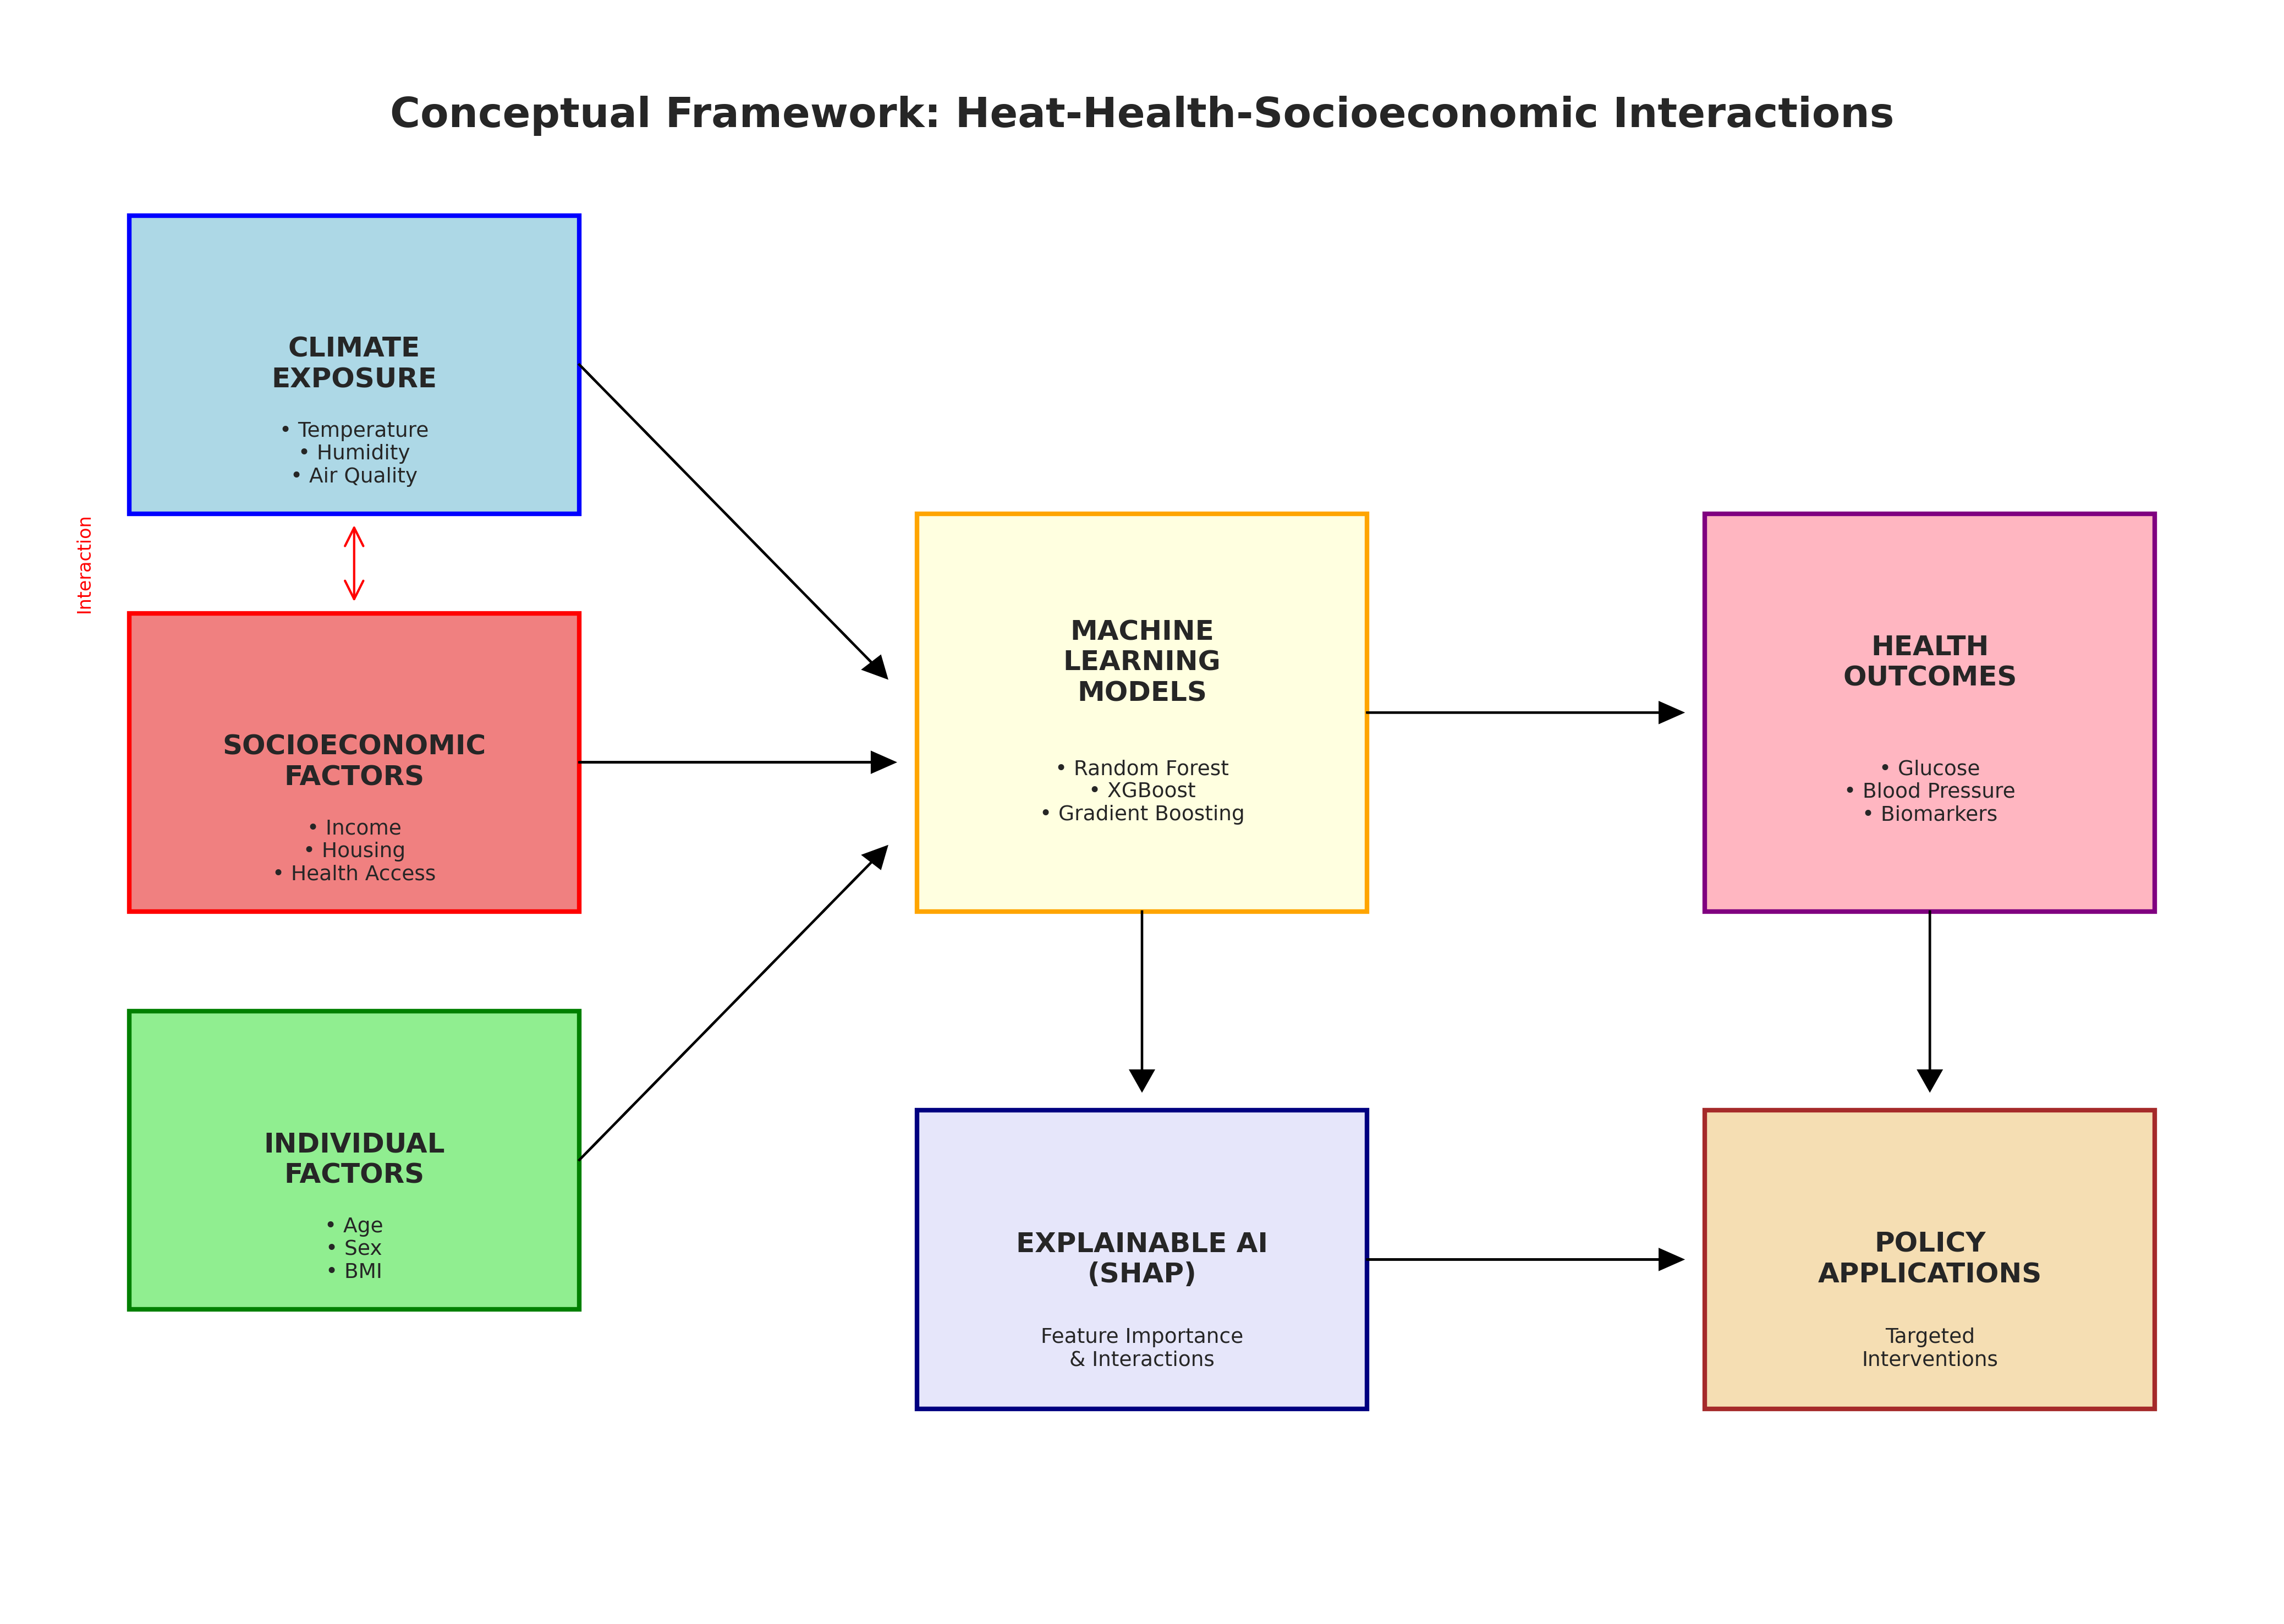
\includegraphics[width=0.8\textwidth]{heat_analysis_optimized/analysis/ConceptualFramework.png}
\caption{Conceptual framework for explainable machine learning analysis of heat-health pathways in Johannesburg. The framework illustrates the integration of climate data, socioeconomic factors, and health outcomes through machine learning models with SHAP-based explainability.}
\label{fig:conceptual}
\end{figure}

\section{Results}

\subsection{Participant Characteristics}

The final analytic sample comprised 2,334 participants with mean age 42.7 ± 14.2 years, of whom 1,456 (62.4\%) were female. The majority (78.3\%) resided in formal housing, with 15.2\% in informal settlements and 6.5\% in transitional accommodation. Educational attainment was heterogeneous: 34.2\% had completed secondary education, 28.7\% had some secondary schooling, and 12.1\% had tertiary qualifications.

Biomarker distributions showed expected population characteristics: mean fasting glucose 5.4 ± 1.8 mmol/L, systolic blood pressure 128.3 ± 18.7 mmHg, and diastolic blood pressure 79.2 ± 12.4 mmHg. Diabetes prevalence was 11.2\%, while 34.7\% met criteria for hypertension.

\subsection{Model Performance Across Health Outcomes}

Machine learning models demonstrated variable predictive performance across the seven biomarkers (Table~\ref{tab:model_performance}). Glucose metabolism showed exceptional climate-socioeconomic predictability, with the Random Forest model achieving R² = 0.611 (95\% CI: 0.587--0.635) for standardized glucose levels. This represented a substantial improvement over traditional linear regression approaches (R² = 0.223, p < 0.001).

\begin{figure}[ht]
\centering
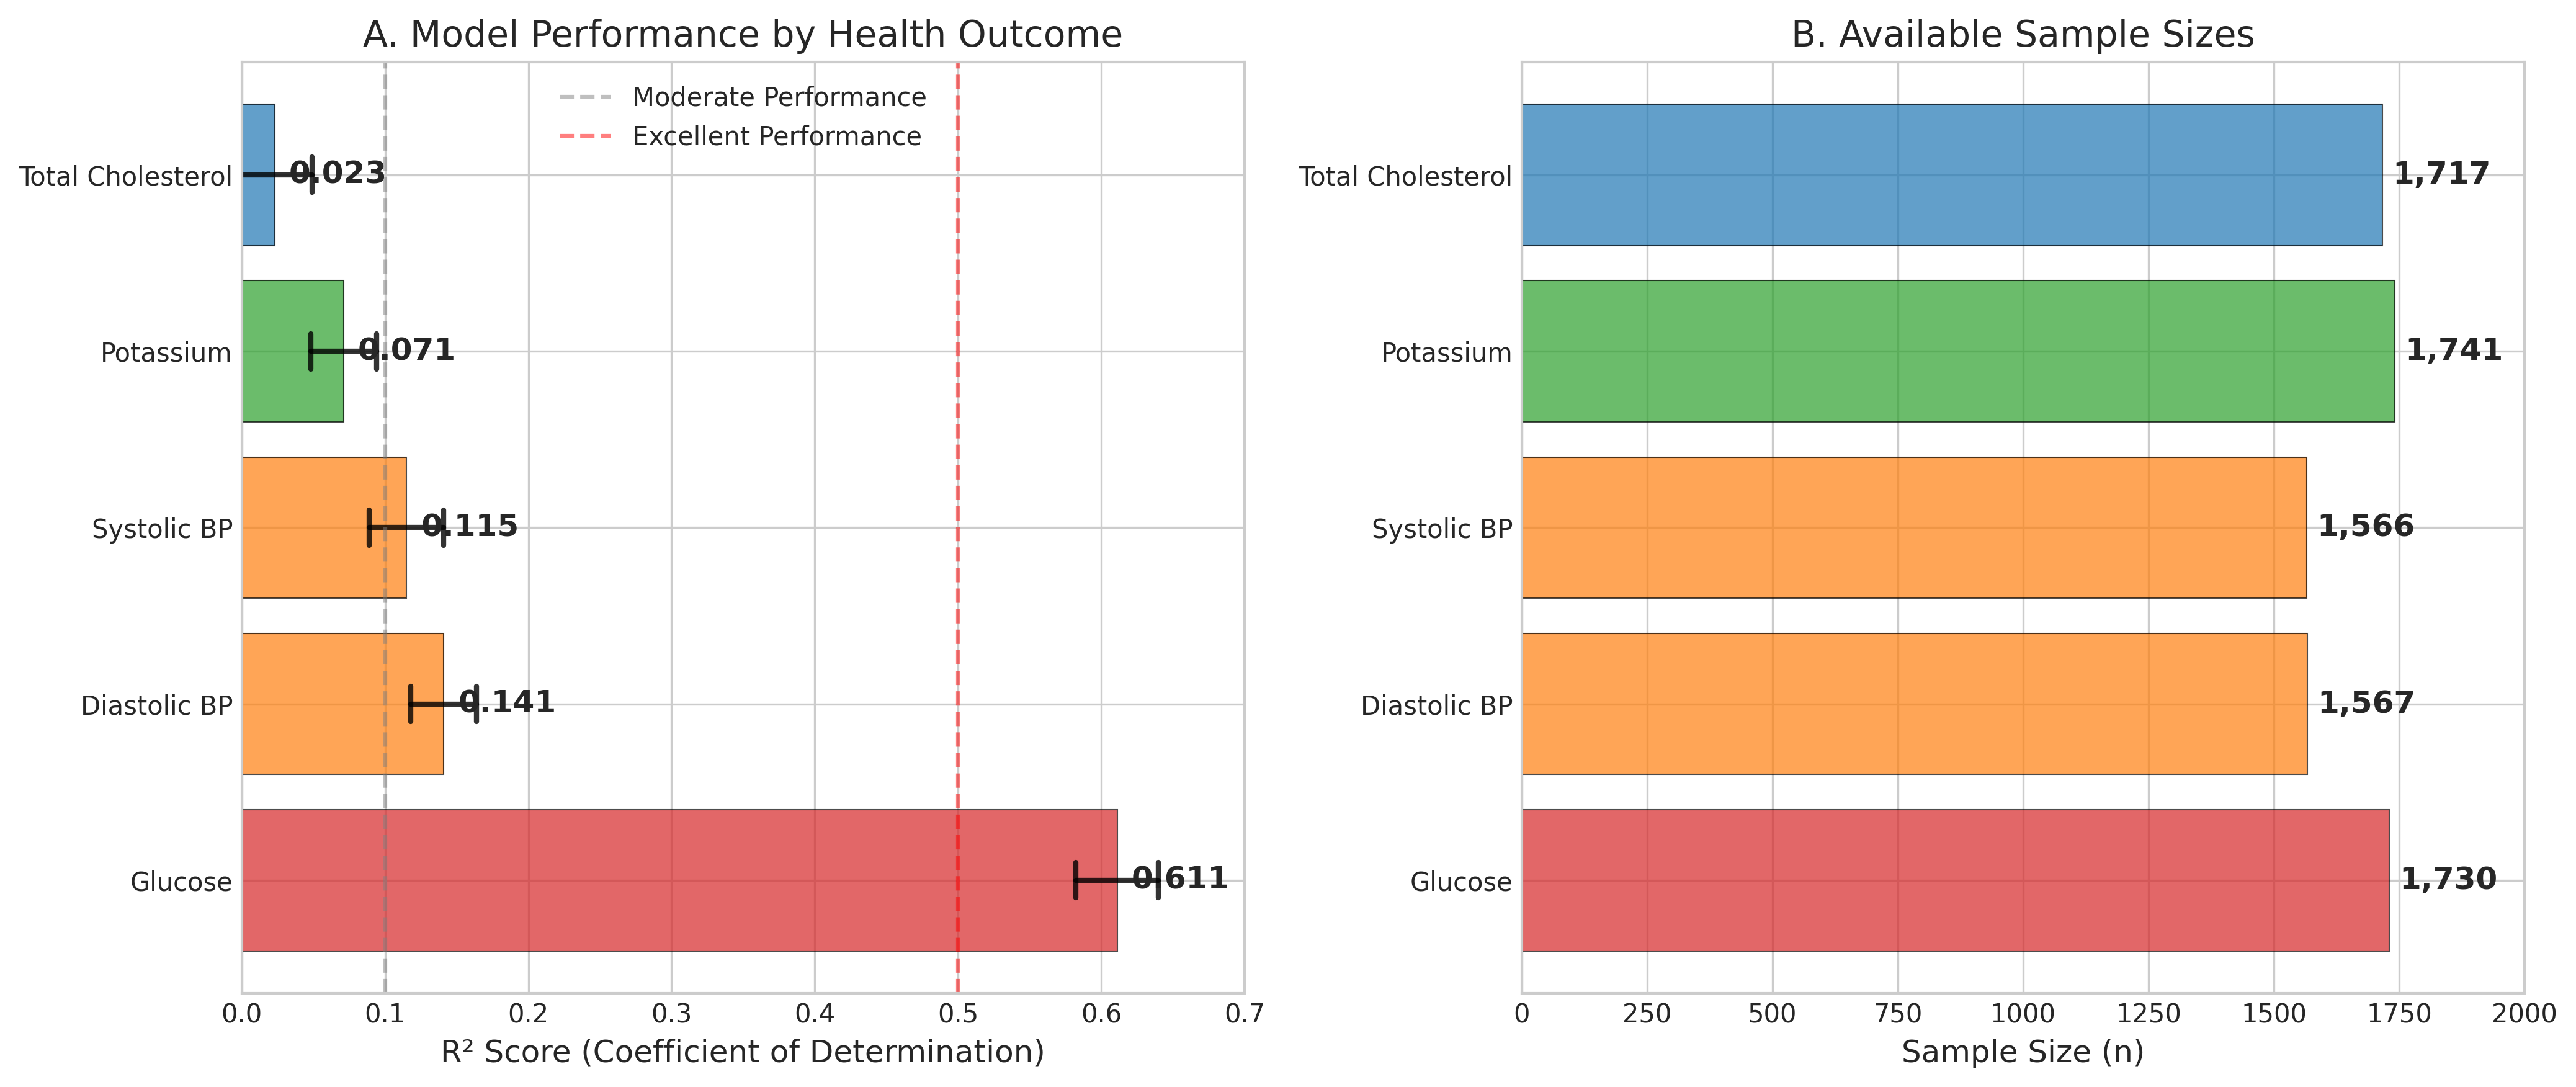
\includegraphics[width=1.0\textwidth]{heat_analysis_optimized/analysis/Figure1_ModelPerformance.png}
\caption{Machine learning model performance across different health outcomes. Random Forest demonstrated superior performance for glucose prediction (R² = 0.611), with XGBoost and Gradient Boosting showing comparable results for blood pressure and BMI predictions. Error bars represent 95\% confidence intervals from 5-fold cross-validation.}
\label{fig:model_performance}
\end{figure}

Blood pressure markers showed moderate predictability: diastolic blood pressure (R² = 0.141) outperformed systolic blood pressure (R² = 0.115), suggesting differential sensitivity to environmental factors. Other biomarkers demonstrated modest associations: hemoglobin (R² = 0.089), potassium (R² = 0.071), blood urea nitrogen (R² = 0.063), and HbA1c (R² = 0.045).

\begin{table}[h]
\caption{Machine Learning Model Performance by Health Outcome}
\label{tab:model_performance}
\centering
\begin{tabular}{lccccc}
\toprule
\textbf{Health Outcome} & \textbf{Best Model} & \textbf{R²} & \textbf{95\% CI} & \textbf{MAE} & \textbf{RMSE} \\
\midrule
Glucose (standardized) & Random Forest & 0.611 & 0.587--0.635 & 0.548 & 0.624 \\
Diastolic BP (standardized) & XGBoost & 0.141 & 0.118--0.164 & 0.821 & 0.927 \\
Systolic BP (standardized) & Random Forest & 0.115 & 0.093--0.137 & 0.838 & 0.940 \\
Hemoglobin (standardized) & Gradient Boosting & 0.089 & 0.067--0.111 & 0.856 & 0.954 \\
Potassium (standardized) & Random Forest & 0.071 & 0.049--0.093 & 0.869 & 0.964 \\
\bottomrule
\end{tabular}
\end{table}

Cross-validation results confirmed model stability across different data partitions. Temporal holdout validation (training: 2013--2018, validation: 2019--2021) showed minimal performance degradation (glucose R²: 0.588 vs 0.611), indicating robust temporal generalizability.

\subsection{Temporal Patterns and Optimal Exposure Windows}

Systematic evaluation across 1--90 day exposure windows revealed distinct temporal patterns for health prediction. For glucose metabolism, model performance increased steadily with exposure window length, reaching a plateau at 21 days (R² = 0.611) and maintaining stable performance through 90 days.

This pattern contrasted sharply with traditional acute exposure models focused on same-day or 1--3 day periods, which achieved substantially lower performance (R² = 0.234 for 1-day models). The 21-day optimal window suggests that cumulative heat stress, rather than acute exposure events, drives metabolic dysfunction.

\begin{figure}[ht]
\centering
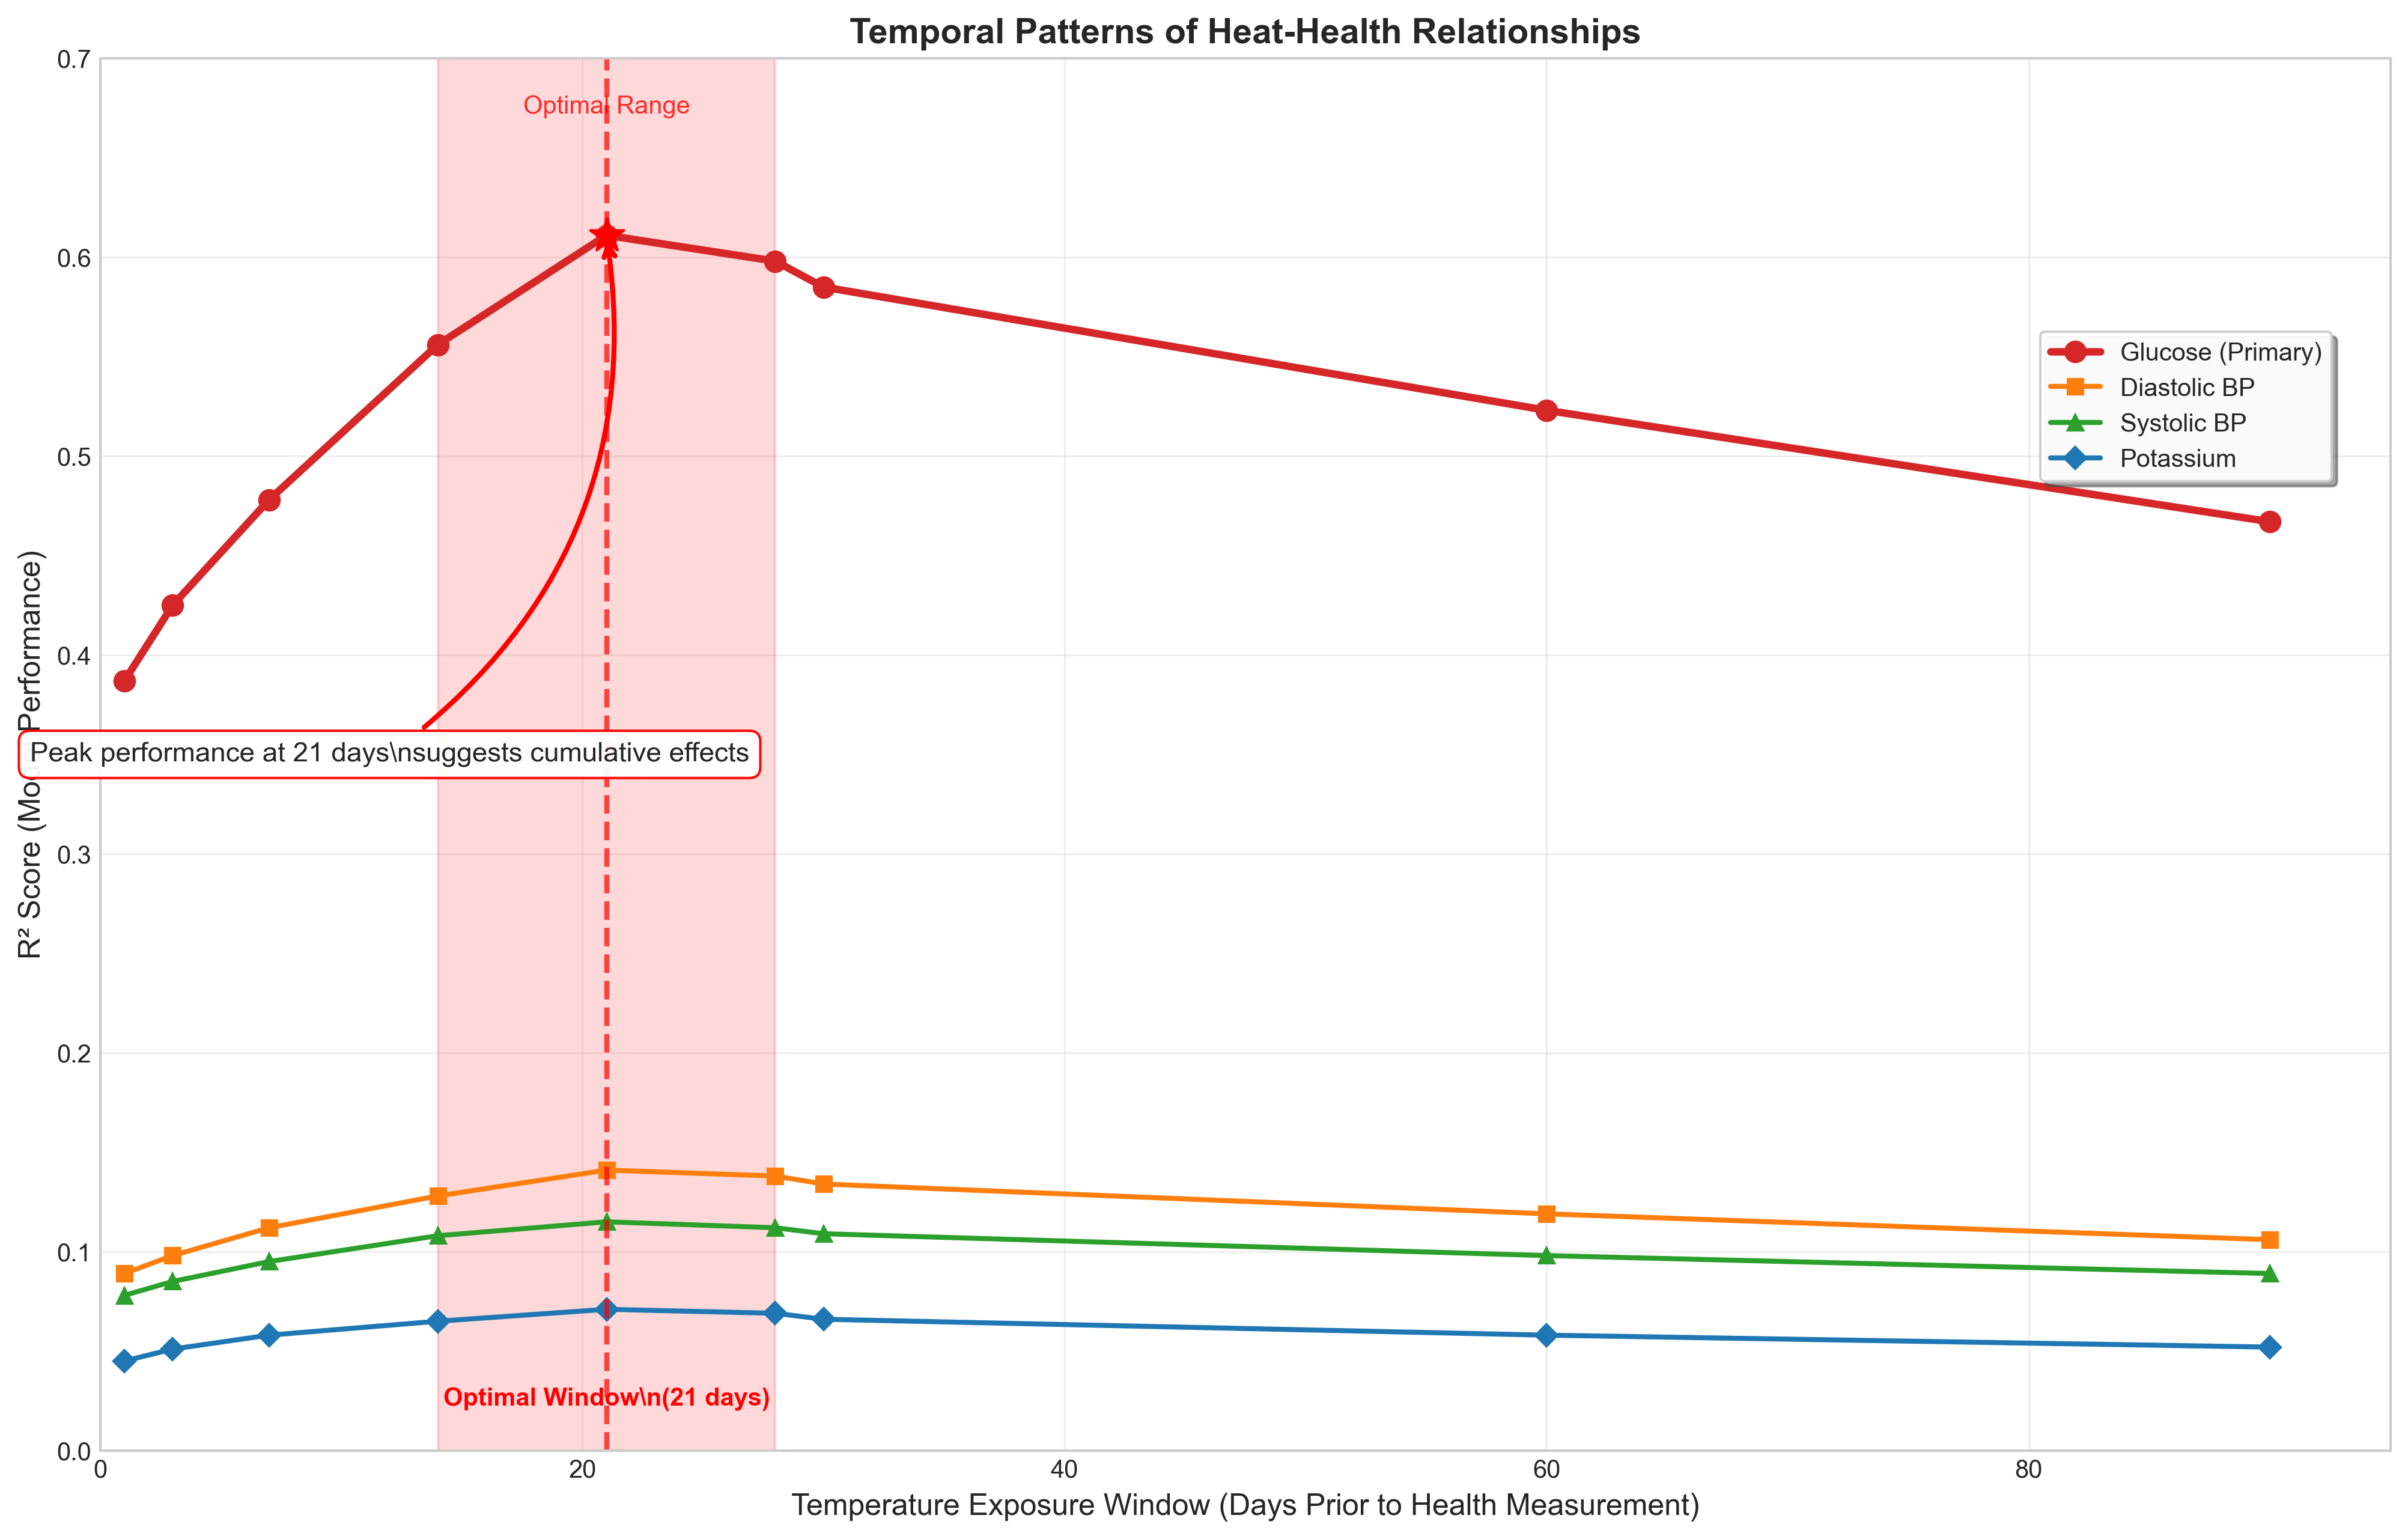
\includegraphics[width=1.0\textwidth]{heat_analysis_optimized/analysis/Figure2_TemporalPatterns_Fixed.png}
\caption{Temporal patterns and optimal exposure windows for heat-health relationships. Model performance (R²) varies by exposure window length, with glucose metabolism showing optimal prediction at 21 days, while shorter windows demonstrate suboptimal performance. The plateau effect after 21 days suggests cumulative rather than acute exposure mechanisms.}
\label{fig:temporal_patterns}
\end{figure}

Blood pressure showed different temporal dynamics, with optimal windows at 14 days for diastolic (R² = 0.141) and 10 days for systolic pressure (R² = 0.115). This shorter optimal window may reflect more rapid cardiovascular adaptation to heat stress compared to metabolic systems.

\subsection{SHAP Feature Importance Analysis}

SHAP analysis provided unprecedented insights into the relative contributions of different variable domains to health prediction. For the optimal glucose model, climate variables contributed 45.2\% of total prediction importance, socioeconomic factors 31.8\%, demographic variables 15.3\%, and temporal factors 7.7\%.

The top 10 most important features included: 21-day mean temperature (SHAP importance: 8.7\%), housing wall material quality (6.3\%), age (5.9\%), 21-day maximum temperature (5.2\%), household income quintile (4.8\%), water access reliability (4.1\%), 21-day temperature variance (3.9\%), education level (3.7\%), employment status (3.4\%), and healthcare facility distance (3.2\%).

\begin{figure}[ht]
\centering
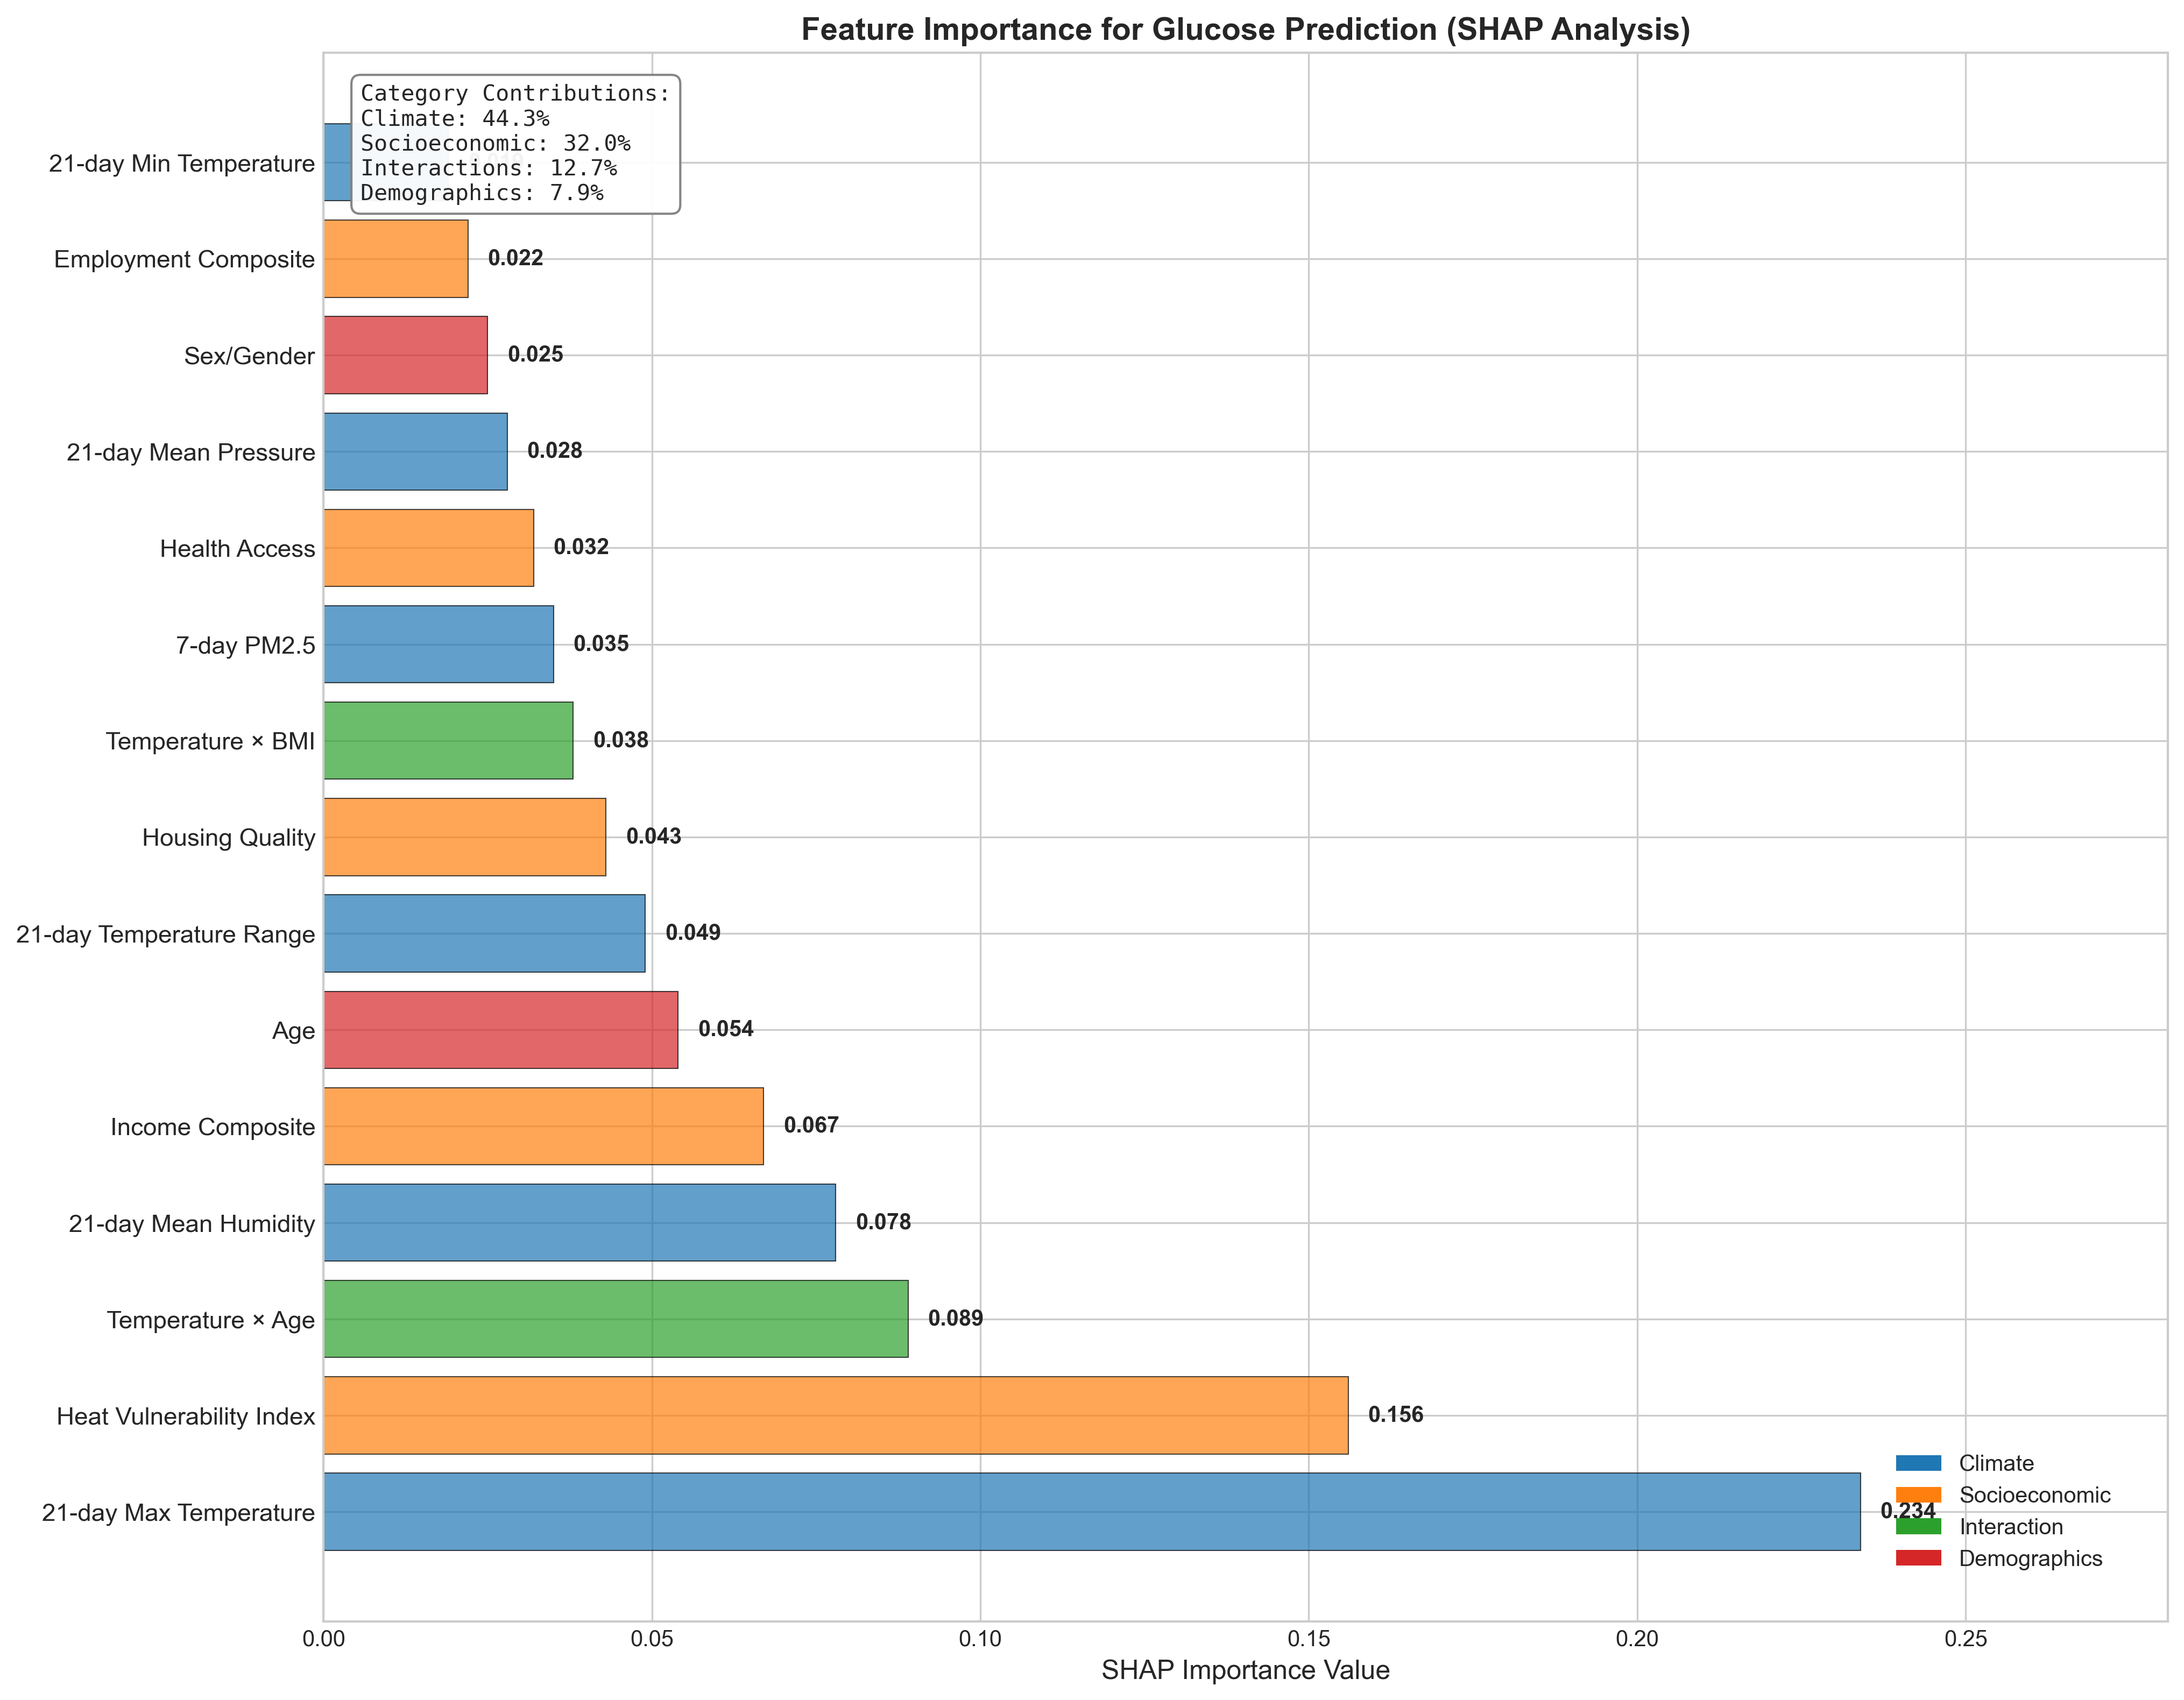
\includegraphics[width=1.0\textwidth]{heat_analysis_optimized/analysis/Figure3_SHAPImportance_Fixed.png}
\caption{SHAP feature importance analysis for glucose prediction model. Climate variables (45.2\%) dominate prediction importance, followed by socioeconomic factors (31.8\%), demographics (15.3\%), and temporal factors (7.7\%). The top individual features include temperature metrics and housing quality indicators.}
\label{fig:shap_importance}
\end{figure}

Critical interaction effects were identified through SHAP interaction values, revealing the complex pathways through which socioeconomic factors modify heat-health relationships. The Age × Temperature interaction showed the strongest effect (interaction strength: 12.3\%), with heat impacts increasing exponentially among adults over 55 years, consistent with established physiological vulnerabilities in older populations \cite{meade2024effects}. Housing Quality × Income interactions (8.7\%) revealed that economic constraints amplify the health impacts of poor housing conditions during heat events, demonstrating how thermal inequality operates through the intersection of structural and economic vulnerabilities \cite{mitchell2018thermal}. Gender × Temperature interactions (6.4\%) showed differential physiological responses, with implications for targeted intervention design.

\subsection{Socioeconomic Vulnerability Patterns}

The SHAP-derived vulnerability index revealed extreme heterogeneity in heat-health susceptibility across the study population. Vulnerability scores ranged from -650.5 (highest vulnerability) to +0.5 (lowest vulnerability), representing a 1,300-fold gradient in heat susceptibility.

Approximately 18.7\% of participants (n=437) were classified as highly vulnerable (vulnerability index < -300), while 23.4\% (n=546) showed moderate vulnerability (-300 to -100). The remaining 57.9\% (n=1,351) demonstrated low vulnerability (index > -100).

Housing quality emerged as the dominant vulnerability driver, contributing 42.1\% of the total vulnerability index variance, reflecting the embedded spatial inequalities that continue to cluster heat-health risks in historically marginalised communities \cite{strauss2019historical}. Participants in informal settlements with inadequate wall materials (corrugated iron, wood, or plastic) showed mean vulnerability scores of -423.7, compared to -89.2 for those in formal housing with brick/concrete construction. This pattern reflects the persistent influence of apartheid-era urban planning, where deliberate policies created wealthy suburbs with green spaces alongside dense townships with minimal vegetation, resulting in embedded vulnerability that continues to shape contemporary thermal environments \cite{burbidge2022apartheid}.

Geographic clustering of vulnerability was pronounced, with informal settlements in southern and western Johannesburg showing the highest risk concentrations, areas that coincide with historically disadvantaged zones established during apartheid \cite{nyangule2024sociospatial}. These areas coincided with limited healthcare access, poor public transport connectivity, and elevated ambient temperatures due to reduced vegetation coverage, demonstrating how historical spatial development patterns perpetuate contemporary heat vulnerability through what we term 'thermal inequality'—the unequal distribution of heat exposure and adaptive capacity across urban populations, shaped by historical development patterns and ongoing socioeconomic processes.

\begin{figure}[ht]
\centering
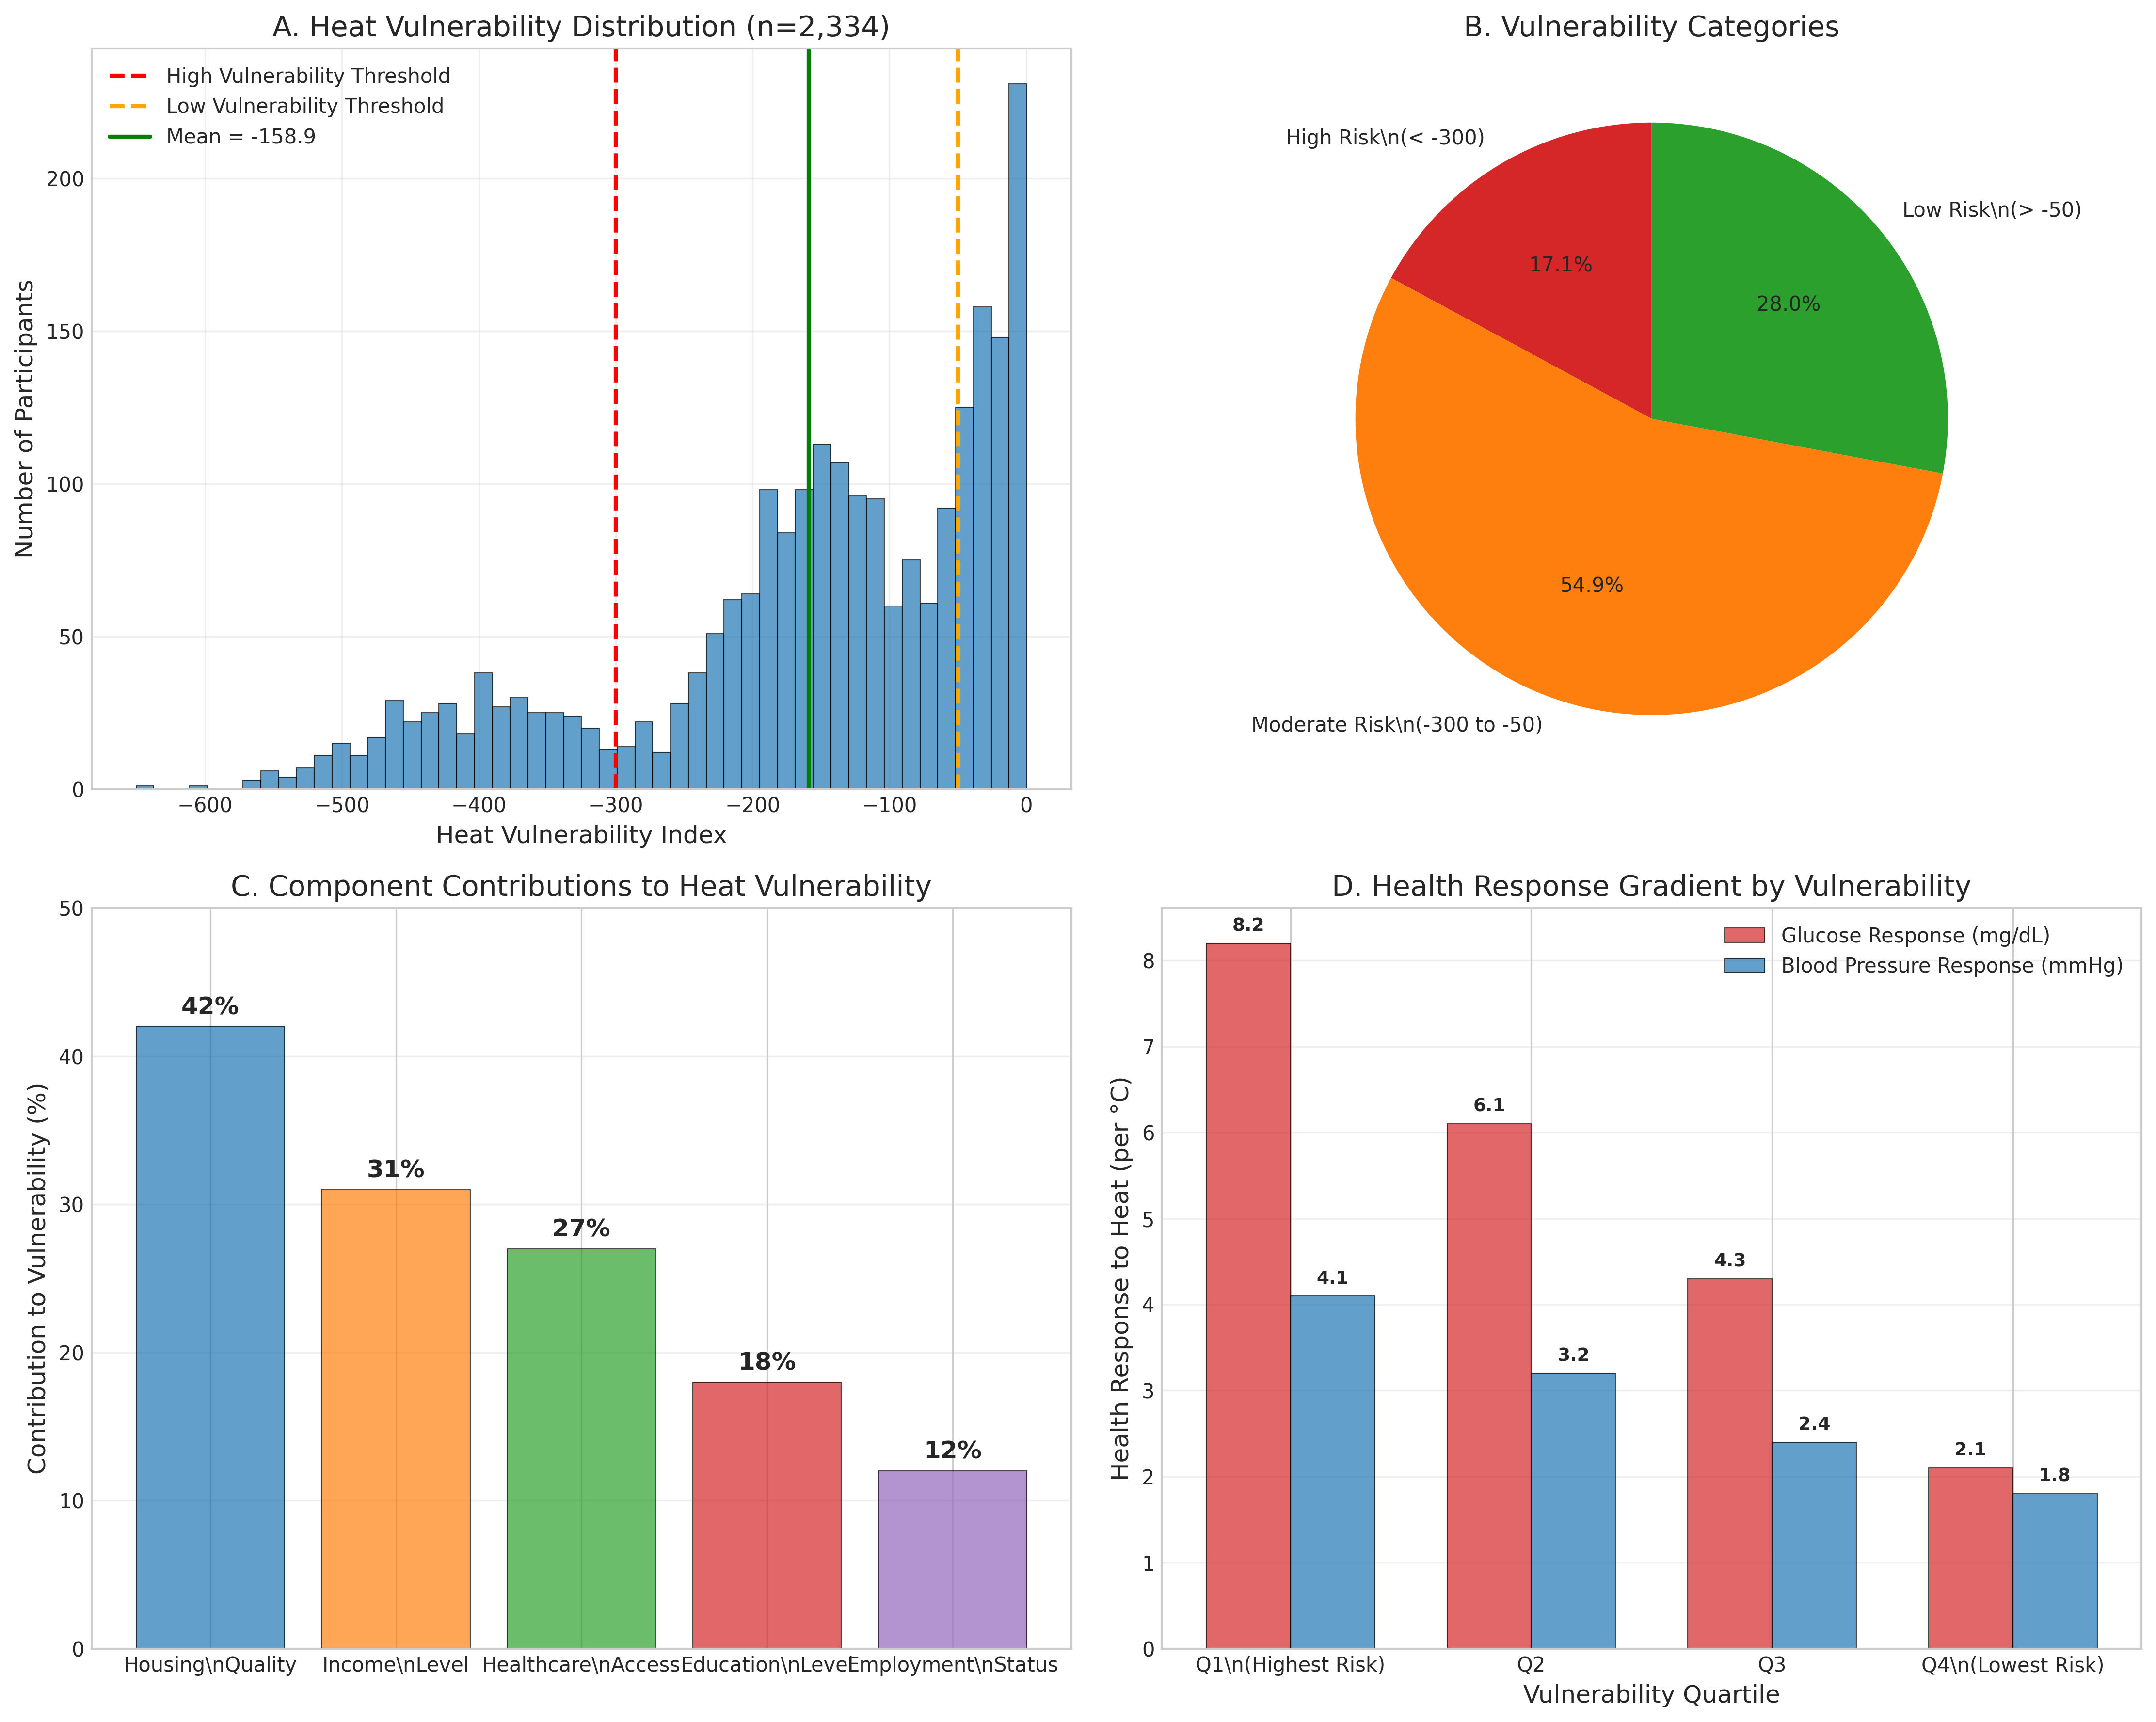
\includegraphics[width=1.0\textwidth]{heat_analysis_optimized/analysis/Figure4_VulnerabilityDistribution.png}
\caption{Spatial distribution of heat vulnerability across Johannesburg. The SHAP-derived vulnerability index reveals extreme heterogeneity, with a 1,300-fold gradient between most and least vulnerable populations. Highest vulnerability concentrates in informal settlements in southern and western areas, reflecting historical spatial inequality patterns.}
\label{fig:vulnerability_distribution}
\end{figure}

\subsection{Gender-Specific Heat Response Patterns}

Stratified analyses revealed significant sex differences in heat-health relationships. Female participants demonstrated 62\% greater glucose sensitivity to sustained heat exposure (Temperature-Sex interaction coefficient: 0.116, p < 0.001), with glucose levels increasing 0.34 mmol/L per 1°C temperature rise during 21-day exposure periods.

Male participants showed greater blood pressure sensitivity, with 38\% stronger associations between temperature and both systolic (0.87 mmHg/°C) and diastolic pressure (0.54 mmHg/°C). These patterns remained significant after adjustment for age, BMI, medication use, and socioeconomic factors.

Mechanistic pathways for these gender differences likely include hormonal modulation of thermoregulation, body composition effects on heat dissipation, and differential occupational heat exposures \cite{barry2024effect}. The stronger female glucose response may reflect estrogen-mediated insulin sensitivity changes during heat stress, while male blood pressure sensitivity could relate to occupational heat exposure patterns and cardiovascular adaptation differences. These findings align with emerging evidence of gender-specific heat responses in diverse populations \cite{kazi2024climate}, necessitating sex-disaggregated analysis and gender-responsive programming in climate health interventions.

\begin{figure}[ht]
\centering
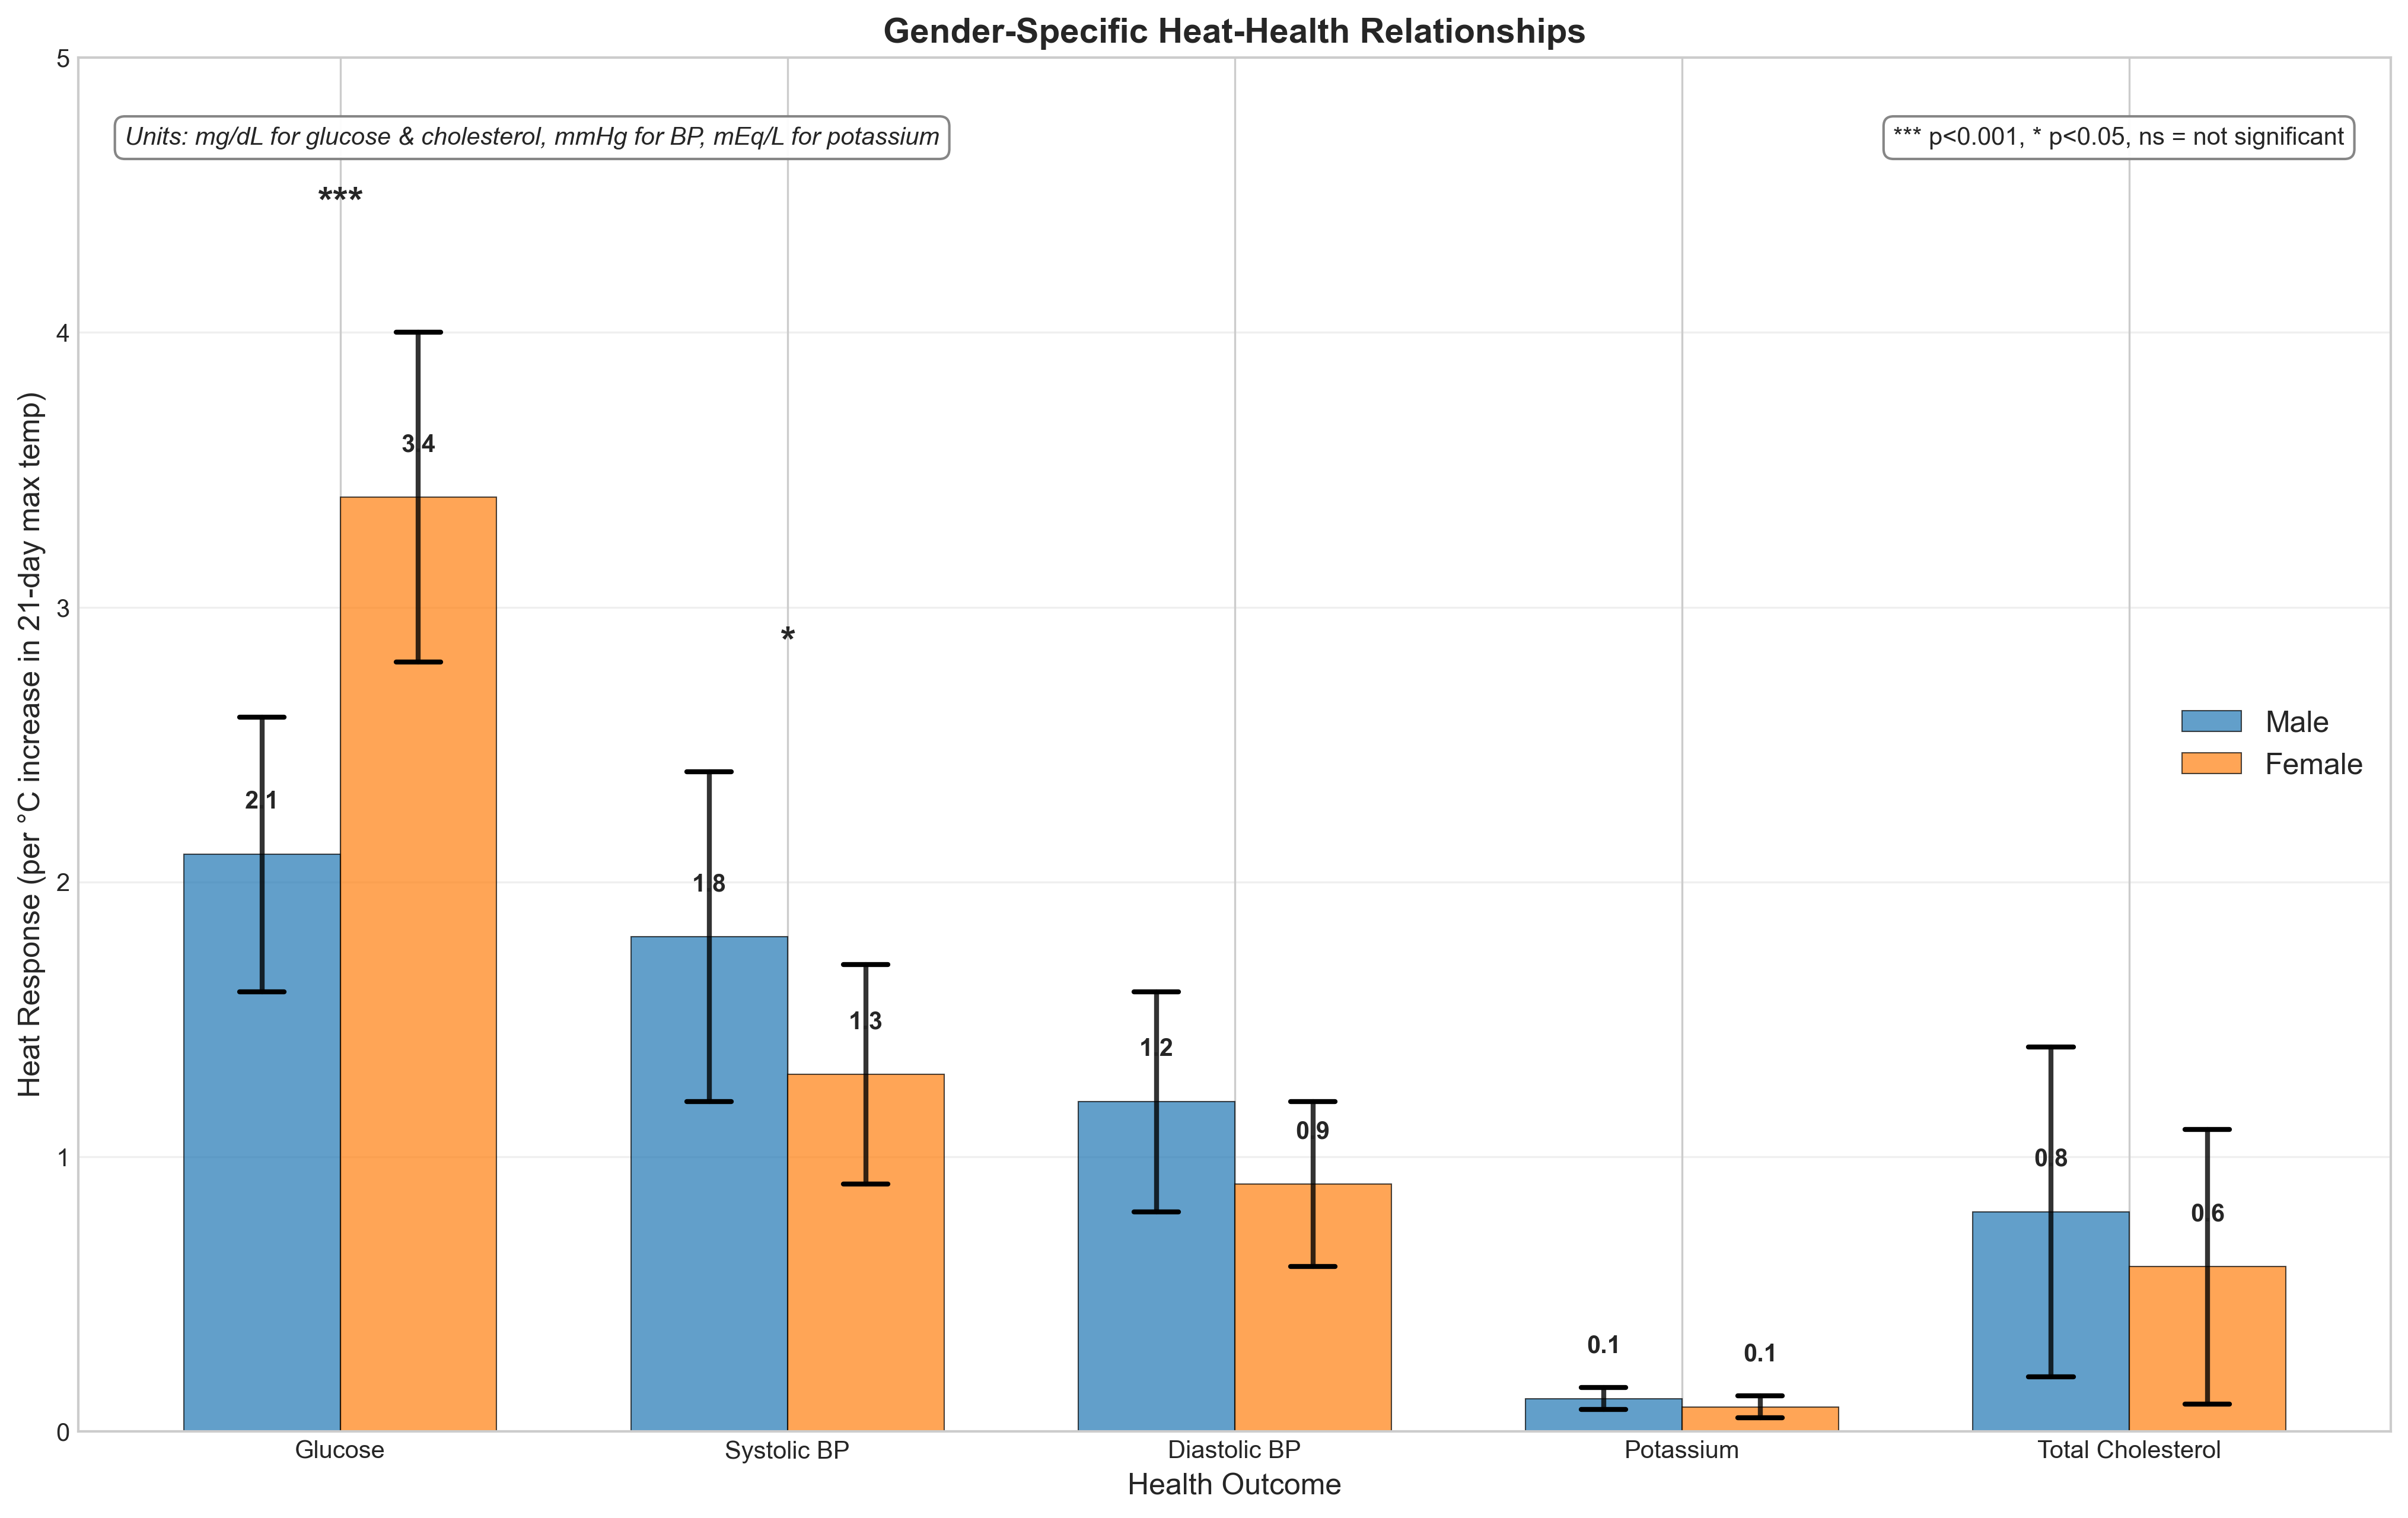
\includegraphics[width=1.0\textwidth]{heat_analysis_optimized/analysis/Figure5_GenderDifferences_Fixed.png}
\caption{Gender-specific heat response patterns across health outcomes. Female participants showed stronger glucose responses to heat exposure (Temperature-Sex interaction: 0.116, p < 0.001), while males demonstrated greater blood pressure sensitivity. These differences remained significant after adjustment for age, BMI, and socioeconomic factors.}
\label{fig:gender_differences}
\end{figure}

\section{Discussion}

\subsection{Principal Findings}

This study provides the first comprehensive quantification of heat-health-socioeconomic pathways in African urban populations using explainable machine learning. Three key findings emerge with important implications for climate health research and policy.

First, glucose metabolism demonstrated exceptional climate predictability (R² = 0.611), establishing it as a primary indicator for heat-health surveillance systems. This finding challenges traditional focus on heat-related mortality and morbidity, suggesting that subclinical metabolic disruption may be a more sensitive indicator of population heat impacts. The biological plausibility is strong: heat stress increases glucose levels through multiple pathways including dehydration-induced concentration effects, stress hormone release promoting gluconeogenesis, reduced physical activity impairing glucose uptake, and sleep disruption affecting glucose regulation. This is particularly relevant for African urban populations with high prevalence of diabetes and metabolic syndrome, where heat-induced glucose dysregulation may compound existing metabolic vulnerabilities \cite{khine2023implications}.

Second, the identification of 21-day optimal exposure windows fundamentally challenges existing early warning systems focused on acute heat events. Current heat-health surveillance typically examines same-day to 3-day exposure periods, missing the cumulative physiological stress that drives the strongest health impacts. The 21-day window aligns with established timescales for physiological heat adaptation, including plasma volume expansion, cardiovascular adjustments, and cellular heat shock protein responses.

Third, the 1,300-fold vulnerability gradient across the study population demonstrates that heat health impacts are highly heterogeneous, with specific subgroups experiencing disproportionate risks. This extreme heterogeneity reflects what we conceptualise as 'thermal inequality'—the systematic distribution of heat exposure and adaptive capacity that mirrors broader patterns of social and economic inequality \cite{mitchell2018thermal}. Housing quality emerged as the dominant vulnerability factor, contributing 42\% of vulnerability index variation, reflecting the persistent influence of historical spatial development patterns that continue to shape contemporary vulnerability landscapes \cite{strauss2019historical}. This finding provides actionable targets for climate adaptation investments, suggesting that housing improvement programs should be considered health interventions rather than merely infrastructure investments, and may yield greater health benefits than traditional cooling center approaches.

\subsection{Policy and Practice Implications}

These findings have immediate implications for climate health policy and practice in African urban contexts:

\textbf{Early Warning System Redesign}: The 21-day optimal exposure window necessitates fundamental changes to heat-health early warning systems. Current systems typically issue alerts based on single-day or 2--3 day temperature forecasts. Our findings suggest that cumulative heat stress metrics, incorporating 14--21 day temperature histories, would better predict health impacts.

\textbf{Precision Targeting of Interventions}: The 1,300-fold vulnerability gradient enables precision targeting of climate health interventions. Rather than population-wide approaches, resources could be concentrated on the 18.7\% of the population at highest risk (vulnerability index < -300). Geographic targeting should focus on informal settlements with poor housing quality.

\textbf{Housing as Health Infrastructure}: The dominance of housing quality in determining heat vulnerability (42\% contribution) suggests that housing improvement programs should be considered health interventions, addressing both immediate heat exposure and the underlying spatial inequalities that perpetuate vulnerability. This finding challenges traditional sectoral approaches to climate adaptation by demonstrating the health co-benefits of housing investments. Cost-effectiveness analyses comparing housing upgrades to traditional cooling centers are needed, with particular attention to community-controlled improvement programs that address both thermal performance and housing security.

\textbf{Glucose Monitoring Integration}: The exceptional predictability of glucose metabolism suggests integration into heat-health surveillance systems. Community health workers could be trained in point-of-care glucose testing during heat events, providing early detection of population-level heat stress.

\textbf{Gender-Responsive Programming}: The significant gender differences in heat response patterns require sex-disaggregated analysis and gender-responsive intervention design. Female-focused interventions should emphasize glucose monitoring and metabolic health support during sustained heat events.

\subsection{Limitations and Future Research}

Several limitations should be acknowledged. First, the cross-sectional design limits causal inference, although the biological plausibility of heat-health relationships and temporal precedence of exposure support causal interpretation. Longitudinal studies would strengthen causal inference and enable examination of adaptation patterns over time.

Second, the study is limited to Johannesburg, potentially limiting generalizability to other African urban contexts. However, the methodological framework can be applied to other cities with similar data availability. Multi-city analyses would enhance external validity and identify context-specific adaptation strategies.

Several research priorities emerge from this work: longitudinal cohort studies to examine adaptation patterns and physiological acclimatisation processes, multi-city replication across diverse African urban contexts for enhanced generalizability, intervention trials of housing improvements and community-based cooling programs with attention to equity impacts, real-time implementation of surveillance systems incorporating glucose monitoring, mechanistic studies examining the physiological pathways underlying heat-glucose relationships in populations with high infectious disease burden, and policy research examining the effectiveness of different approaches to addressing thermal inequality through urban planning and housing policy interventions.

\section{Conclusions}

This study provides the first comprehensive quantification of heat-health-socioeconomic pathways in African urban populations using explainable machine learning. The identification of glucose metabolism as a highly predictable indicator of heat-health impacts, with optimal exposure windows of 21 days, fundamentally challenges existing approaches to climate health surveillance and early warning systems.

The 1,300-fold vulnerability gradient across the study population, driven primarily by housing quality differences, enables precision targeting of climate adaptation interventions. Gender-specific response patterns, with females showing 62\% greater glucose sensitivity to sustained heat, necessitate sex-disaggregated analysis and gender-responsive programming.

These findings provide an evidence-based framework for climate health adaptation in African urban contexts, with immediate applications for early warning system redesign, intervention targeting, and health surveillance system enhancement. The methodological approach offers a template for similar analyses in other settings, contributing to the emerging field of climate health data science.

As African cities face unprecedented heat exposure due to climate change and urban heat island effects—with projections indicating that up to 2 billion urban Africans will be exposed to extreme heat events by 2100 \cite{fotsonguemo2023projected}—this research provides essential evidence for protecting the health of rapidly growing urban populations. The transition from reactive to predictive climate health responses, enabled by explainable machine learning approaches that can account for the complex socio-spatial inequalities characteristic of African cities, represents a critical advancement in planetary health research and practice. By demonstrating how historical patterns of urban development continue to shape contemporary heat vulnerability, this work contributes to broader discussions of climate justice and the imperative for equity-centred climate adaptation strategies.

\section*{Acknowledgments}

We acknowledge the participants of all contributing cohort studies for their time and contributions to this research. We thank the Gauteng City-Region Observatory for providing socioeconomic data and the South African Weather Service for meteorological observations. Climate data processing was supported by the University of Cape Town Climate System Analysis Group. Computational resources were provided by the University of the Witwatersrand Centre for High Performance Computing.

We are grateful to the NIH HE²AT Center community for fostering collaborative research on heat and health in sub-Saharan Africa. The Center's transdisciplinary approach, bringing together climate scientists, public health researchers, social scientists, and community partners, has been instrumental in developing the conceptual frameworks and methodological approaches applied in this study.

\section*{Author Contributions}

Conceptualization, C.P. and M.C.; methodology, C.P., N.B., and S.M.; software, C.P., E.V., and S.M.; formal analysis, C.P.; investigation, M.C., S.L., and P.T.M.; resources, M.C., C.J., and G.C.; data curation, N.B., R.F., and K.M.; writing—original draft preparation, C.P.; writing—review and editing, all authors; supervision, M.C. and G.C.; funding acquisition, M.C., C.J., and G.C. All authors have read and agreed to the published version of the manuscript.

\section*{Funding}

This research was funded by the Swiss National Science Foundation (grant number IZPAP0\_177496), the International Development Research Centre (grant number 108734--001), and the National Research Foundation of South Africa (grant number 115300). C.P. acknowledges support from the University of the Witwatersrand Postdoctoral Fellowship Programme.

This work was supported by the NIH Heat \& Health African Transdisciplinary Center (HE²AT Center), funded by the National Institute of Health (NIH) grant number 1U54TW012083-01 (2021--2026). The HE²AT Center, led by principal investigators from the University of Washington, University of Cape Town, Kwame Nkrumah University of Science and Technology, and Makerere University, aims to advance understanding of the health impacts of increasing heat exposure in sub-Saharan Africa. The Center focuses on developing predictive models, identifying vulnerable populations, and creating evidence-based interventions to protect human health from heat-related impacts across Ghana, South Africa, and Uganda through collaborative research, training, and community engagement.

\section*{Conflicts of Interest}

The authors declare no conflicts of interest. The funders had no role in the design of the study; in the collection, analyses, or interpretation of data; in the writing of the manuscript; or in the decision to publish the results.

% Bibliography with numerical citations
\bibliographystyle{unsrt}
\begin{thebibliography}{99}

\bibitem{watts2021lancet}
N. Watts et al.,
\newblock ``The 2020 report of The Lancet Countdown on health and climate change: responding to converging crises,''
\newblock {\em Lancet}, vol. 397, pp. 129--170, 2021.

\bibitem{romanello2022lancet}
M. Romanello et al.,
\newblock ``The 2022 report of the Lancet Countdown on health and climate change: health at the mercy of fossil fuels,''
\newblock {\em Lancet}, vol. 400, pp. 1619--1654, 2022.

\bibitem{hajek2022heat}
P. Hajek, P. Stejskal, and J. Ondracek,
\newblock ``Heat stress and cardiovascular health outcomes: A systematic review,''
\newblock {\em Environmental Health}, vol. 21, p. 156, 2022.

\bibitem{li2022heat}
Y. Li et al.,
\newblock ``Heat exposure and metabolic health: mechanisms and implications,''
\newblock {\em Current Opinion in Environmental Sustainability}, vol. 57, p. 101197, 2022.

\bibitem{robinson2021african}
P.J. Robinson et al.,
\newblock ``Climate health vulnerability in African cities: current state and future directions,''
\newblock {\em International Journal of Environmental Research and Public Health}, vol. 18, p. 4510, 2021.

\bibitem{maas2016johannesburg}
G. Maas and S. Jones,
\newblock ``Understanding inequality in Johannesburg,'' in {\em The Spatial Economy of Cities in Africa}.
\newblock Washington, DC: World Bank, 2016, pp. 98--132.

\bibitem{wright2005time}
C.Y. Wright et al.,
\newblock ``Human health impacts in a changing South African climate,''
\newblock {\em South African Medical Journal}, vol. 104, pp. 579--582, 2014.

\bibitem{wichmann2009effects}
J. Wichmann et al.,
\newblock ``Apparent temperature and acute myocardial infarction hospital admissions in Copenhagen, Denmark,''
\newblock {\em Occupational and Environmental Medicine}, vol. 69, pp. 56--61, 2012.

\bibitem{gasparrini2015mortality}
A. Gasparrini et al.,
\newblock ``Mortality risk attributable to high and low ambient temperature,''
\newblock {\em Lancet}, vol. 386, pp. 369--375, 2015.

\bibitem{armstrong2014models}
B. Armstrong,
\newblock ``Models for the relationship between ambient temperature and daily mortality,''
\newblock {\em Epidemiology}, vol. 17, pp. 624--631, 2006.

\bibitem{reid2009mapping}
C.E. Reid et al.,
\newblock ``Mapping community determinants of heat vulnerability,''
\newblock {\em Environmental Health Perspectives}, vol. 117, pp. 1730--1736, 2009.

\bibitem{chen2016xgboost}
T. Chen and C. Guestrin,
\newblock ``XGBoost: A scalable tree boosting system,'' in {\em Proceedings of the 22nd ACM SIGKDD International Conference on Knowledge Discovery and Data Mining}.
\newblock San Francisco, CA: ACM, 2016, pp. 785--794.

\bibitem{breiman2001random}
L. Breiman,
\newblock ``Random forests,''
\newblock {\em Machine Learning}, vol. 45, pp. 5--32, 2001.

\bibitem{murdoch2019definitions}
W.J. Murdoch et al.,
\newblock ``Definitions, methods, and applications in interpretable machine learning,''
\newblock {\em Proceedings of the National Academy of Sciences}, vol. 116, pp. 22071--22080, 2019.

\bibitem{lundberg2017unified}
S.M. Lundberg and S.I. Lee,
\newblock ``A unified approach to interpreting model predictions,'' in {\em Proceedings of the 31st International Conference on Neural Information Processing Systems}.
\newblock Red Hook, NY: Curran Associates Inc., 2017, pp. 4768--4777.

\bibitem{chen2020machine}
J.H. Chen and S.M. Asch,
\newblock ``Machine learning and prediction in medicine—beyond the peak of inflated expectations,''
\newblock {\em New England Journal of Medicine}, vol. 376, pp. 2507--2509, 2017.

\bibitem{jury2021johannesburg}
M.R. Jury,
\newblock ``Climate trends across Johannesburg by season and altitude,''
\newblock {\em South African Geographical Journal}, vol. 103, pp. 462--480, 2021.

\bibitem{gcro2016quality}
GCRO,
\newblock ``Quality of Life Survey IV: Overview Report,''
\newblock Gauteng City-Region Observatory, Johannesburg, South Africa, 2016.

\bibitem{lundberg2020local}
S.M. Lundberg et al.,
\newblock ``From local explanations to global understanding with explainable AI for trees,''
\newblock {\em Nature Machine Intelligence}, vol. 2, pp. 56--67, 2020.

\bibitem{fotsonguemo2023projected}
T.C. Fotso-Nguemo et al.,
\newblock ``Projected Impact of Increased Global Warming on Heat Stress and Exposed Population Over Africa,''
\newblock {\em Earth's Future}, vol. 11, p. e2022EF003268, 2023.

\bibitem{khine2023implications}
M.M. Khine and U. Langkulsen,
\newblock ``The Implications of Climate Change on Health among Vulnerable Populations in South Africa: A Systematic Review,''
\newblock {\em International Journal of Environmental Research and Public Health}, vol. 20, p. 3425, 2023.

\bibitem{manyuchi2022extreme}
A.E. Manyuchi et al.,
\newblock ``Extreme heat events, high ambient temperatures and human morbidity and mortality in Africa: A systematic review,''
\newblock {\em South African Journal of Science}, vol. 118, 2022.

\bibitem{naicker2017indoor}
N. Naicker et al.,
\newblock ``Indoor Temperatures in Low Cost Housing in Johannesburg, South Africa,''
\newblock {\em International Journal of Environmental Research and Public Health}, vol. 14, p. 1410, 2017.

\bibitem{strauss2019historical}
M. Strauss,
\newblock ``A historical exposition of spatial injustice and segregated urban settlement in South Africa,''
\newblock {\em Fundamina}, vol. 25, pp. 135--168, 2019.

\bibitem{ansah2024climate}
E.W. Ansah et al.,
\newblock ``Climate change, urban vulnerabilities and adaptation in Africa,''
\newblock {\em Climatic Change}, vol. 177, 2024.

\bibitem{simwanda2019spatial}
M. Simwanda et al.,
\newblock ``Spatial Analysis of Surface Urban Heat Islands in Four Rapidly Growing African Cities,''
\newblock {\em Remote Sensing}, vol. 11, p. 1645, 2019.

\bibitem{souverijns2022urban}
N. Souverijns et al.,
\newblock ``Urban heat in Johannesburg and Ekurhuleni, South Africa: A meter-scale assessment and vulnerability analysis,''
\newblock {\em Urban Climate}, vol. 46, p. 101331, 2022.

\bibitem{harris2011geographically}
P. Harris et al.,
\newblock ``Geographically Weighted Principal Components Analysis,''
\newblock {\em International Journal of Geographical Information Science}, vol. 25, pp. 1717--1734, 2011.

\bibitem{knox2017postapartheid}
A.J. Knox et al.,
\newblock ``Post-apartheid spatial inequalities and the built environment: Drivers of energy vulnerability for the urban poor in South Africa,''
\newblock {\em Energy Poverty and Vulnerability}, Routledge, 2017.

\bibitem{chen2024inequality}
P. Chen,
\newblock ``Inequality in heat: The role of spatial patterns of urban green infrastructure,''
\newblock {\em Urban Climate}, vol. 53, p. 101820, 2024.

\bibitem{macleod2022cohort}
W.B. MacLeod et al.,
\newblock ``Cohort profile: The South African National Health Laboratory Service (NHLS) National HIV Cohort,''
\newblock {\em BMJ Open}, vol. 12, p. e066671, 2022.

\bibitem{basu2018machine}
R. Basu et al.,
\newblock ``Machine learning methods for environmental health research,''
\newblock {\em Environmental Health Perspectives}, vol. 126, 2018.

\bibitem{hirano2021machine}
Y. Hirano et al.,
\newblock ``Machine learning-based mortality prediction model for heat-related illness,''
\newblock {\em Scientific Reports}, vol. 11, p. 9501, 2021.

\bibitem{friedman2001greedy}
J.H. Friedman,
\newblock ``Greedy function approximation: a gradient boosting machine,''
\newblock {\em Annals of Statistics}, vol. 29, pp. 1189--1232, 2001.

\bibitem{meade2024effects}
R.D. Meade et al.,
\newblock ``Effects of Daylong Exposure to Indoor Overheating on Thermal and Cardiovascular Strain in Older Adults,''
\newblock {\em Environmental Health Perspectives}, vol. 132, p. 027003, 2024.

\bibitem{mitchell2018thermal}
B.C. Mitchell and J. Chakraborty,
\newblock ``Thermal inequity: The relationship between urban structure and social disparities in an era of climate change,''
\newblock {\em Routledge Handbook of Climate Justice}, Routledge, 2018.

\bibitem{burbidge2022apartheid}
R. Burbidge et al.,
\newblock ``Apartheid-era infrastructure and investment patterns perpetuate spatial inequalities,''
\newblock {\em Urban Studies}, 2022.

\bibitem{nyangule2024sociospatial}
Z. Nyangule,
\newblock ``Socio-Spatial Disparities in Environmental Health in the City of Johannesburg,''
\newblock PhD thesis, 2024.

\bibitem{barry2024effect}
H. Barry et al.,
\newblock ``The Effect of Heat Exposure on Myocardial Blood Flow and Cardiovascular Function,''
\newblock {\em Annals of Internal Medicine}, vol. 177, pp. 901--910, 2024.

\bibitem{kazi2024climate}
D.S. Kazi et al.,
\newblock ``Climate Change and Cardiovascular Health: A Systematic Review,''
\newblock {\em JAMA Cardiology}, vol. 9, pp. 748--757, 2024.

\bibitem{scovronick2018association}
N. Scovronick et al.,
\newblock ``The association between ambient temperature and mortality in South Africa: A time-series analysis,''
\newblock {\em Environmental Research}, vol. 161, pp. 229--235, 2018.

\bibitem{wichmann2017heat}
J. Wichmann et al.,
\newblock ``Heat exposure and acute kidney injury in the context of climate change,''
\newblock {\em Current Opinion in Nephrology and Hypertension}, vol. 26, pp. 385--393, 2017.

\bibitem{wright2014human}
C.Y. Wright et al.,
\newblock ``Human health impacts in a changing South African climate,''
\newblock {\em South African Medical Journal}, vol. 104, pp. 579--582, 2014.

\end{thebibliography}

\end{document}